\documentclass{IEEEcsmag}

\usepackage[colorlinks,urlcolor=blue,linkcolor=blue,citecolor=blue]{hyperref}

\usepackage{xcolor}
\definecolor{bemppgrey}{HTML}{555555}
\definecolor{bempporange}{HTML}{FF7A1A}

\usepackage{pythonhighlight}

\usepackage{tikz}
\usetikzlibrary{arrows,decorations.pathreplacing}
\usepackage{ifthen}

\usepackage{upmath}
\usepackage{upgreek}
\usepackage{amsmath, amssymb}

\usepackage{cleveref}
\crefname{equation}{Equation}{Equations}
\Crefname{equation}{Equation}{Equations}
\crefname{figure}{Figure}{Figures}
\Crefname{figure}{Figure}{Figures}
\crefname{section}{Section}{Sections}
\Crefname{section}{Section}{Sections}

% Bold vector (for points in R^3)
\newcommand{\bvec}[1]{\boldsymbol{#1}}
\def\bx{\bvec{x}}
\def\by{\bvec{y}}
\newcommand{\ds}[1][]{\,\mathrm{d}s\ifthenelse{\equal{#1}{}}{}{_{#1}}}

% Discrete vector and discrete matrix
\newcommand{\dmat}[1]{\mathbf{#1}}
\newcommand{\dvec}[1]{\mathbf{#1}}

\newcommand{\ii}{\mathrm{i}}
\newcommand{\ee}{\mathrm{e}}


\jvol{XX}
\jnum{XX}
\paper{8}
\jmonth{May/June}
\jname{IT Professional}
\pubyear{2021}
\newtheorem{theorem}{Theorem}
\newtheorem{lemma}{Lemma}

\setcounter{secnumdepth}{0}

\begin{document}

\sptitle{Department: Head}
\editor{Editor: Name, xxxx@email}

\title{Designing a high-performance boundary element library with OpenCL and Numba}

\author{T. Betcke}
\affil{Department of Mathematics, University College London}

\author{M. W. Scroggs}
\affil{Department of Engineering, University of Cambridge}

\markboth{Department Head}{Paper title}

\begin{abstract}
The Bempp boundary element library is a well known library for the simulation of a range of electrostatic, acoustic and electromagnetic problems in homogeneous bounded and unbounded domains. It originally started as a traditional C++ library with a Python interface. Over the last two years we have completely redesigned Bempp as a native Python library, called Bempp-cl, that provides computational backends for OpenCL (using PyOpenCL) and Numba. The OpenCL backend implements kernels for GPUs and CPUs with SIMD optimization. In this paper, we discuss the design of Bempp-cl, provide performance comparisons on different compute devices, and discuss the advantages and disadvantages of OpenCL as compared to Numba.
\end{abstract}

\maketitle

\chapterinitial{The Bempp boundary element library} (originally named BEM++) started in 2011 as a project to develop an open-source C++ library for the fast solution of boundary integral equations. The original release came with a simple Python wrapper to the C++ library. Over time, more and more functionality was moved into the Python interface, while computationally intensive routines and the main data structures remained in C++.

At the end of 2019, we completed the main steps of a full rewrite of Bempp and released the first version (0.1) of Bempp-cl \cite{Bempp-cl}. This was followed later in 2020 by version 0.2, the first release that we considered feature complete and mature for application use. Since then we have used Bempp-cl in a number of practical applications and many of our users are migrating to it from the old C++ based Bempp. In this article, we discuss the motivation for the rewrite and restructure of Bempp and the reasoning behind the design choices we made when writing Bempp-cl.

\subsection{The three language problem}
The original BEM++ was troubled by what is often called the two language problem. It is common for programming language to be either easy for humans to write (e.g., Python) or easy for computers to run and acheive high performance (e.g., C++). It is not common, however, for a language to do both of these. Due to this, it is common in scientific computing libraries to write a library in a fast low-level language such as C++, while providing a user interface in a higher-level language such as Python.

This was the model followed by BEM++, but the problem would perhaps better be described as a three language problem: as well as the Python and C++ code contained in libraries like this, it is common to also include a significant amount of code in a third interfacing language. In the case of BEM++, this third language was Cython, an extension of Python with C data types that can be compiled to include functionality from C++ libraries.

Due to the three languages involved, making changes to the library would often mean having to duplicate changed in three places, with many class structures duplicated in all three languages. This made seemingly simple changes in onorous tasks, and provided a barrier to new members of the community looking to contribute to the open-source project.

\subsection{Delegating computations with PyOpenCL}
Prompted by a desire to simplify the library as well as to be able to run on a wide range of CPU and GPU devices, we began a full re-write in 2018, which led to Bempp-cl. The aims of this rewrite were to support explicit single-instruction-multiple-data (SIMD) optimization on CPUs with various instruction lengths, be able to offload computations to AMD, Intel, and Nvidia GPUs, and to base the complete codebase on Python. These aims naturally led to the choice of building a Python library based around OpenCL (using the PyOpenCL interface) and Numba.

In addition to the performance benefits, the library redesign has greatly improved the issues related to the three language problem. Both OpenCL and Numba are use to compile functions. Each function is provided all the data is needs as inputs, so there is no need to duplicate any class structure outside Python. The need for a third interfacing language is removed, as the interfacing to the OpenCL kernels is handled by PyOpenCL.

Boundary element methods are particularly suited to this library model, as the main performance critical task is the computation of discrete operators. Once fast kernels for this have been implemented, the remaining functionality of the library can be written entirely in Python without any great decrease in performance.

\bigskip

We begin this article by giving an overview of the boundary element method, and looking at how Bempp can be used to implement such problems. Following this, we discuss the implementation of boundary element kernels using OpenCL in more detail, and provide a number of performance benchmarks on different compute devices, including CPUs, AMD, Intel, and Nvidia GPUs.


\section{Boundary element methods with Bempp}
In this section, we provide a brief introduction to boundary element methods and describe the necessary steps for their numerical discretisation and solution.

The most simple boundary integral equation is of the form
\begin{align}
  \label{eq:bnd_integral}
  \int_{\Gamma} g(\bx, \by)\phi(\by)\ds[\by] &= f(\bx),&&\bx\in\Gamma.
\end{align}
The function $g(\bx, \by)$ is a Green's function, $f$ is a given right-hand side, and $\phi$ is an unknown surface density over the boundary $\Gamma$ of a bounded three dimensional domain $\Omega\subset\mathbb{R}^3$.

As a concrete example, we consider computing the electrostatic capacity of an object $\Omega$. In this case, we solve the above equation with $f(\bx)=1$ and $g(\bx,\by)=\frac{1}{4\uppi|\bx - \by|}$. Once $\phi$ has been found, the normalised capacity is then obtained using $c = \frac{1}{4\uppi}\int_{\Gamma}\phi(\bx)\ds[\bx]$.

Many practical problems have a significantly more complex structure and can involve block systems of integral equations. Nevertheless, the fundamental structure of what Bempp-cl does is well described by the above problem and will be described in the following.

\begin{figure}
  \centering
  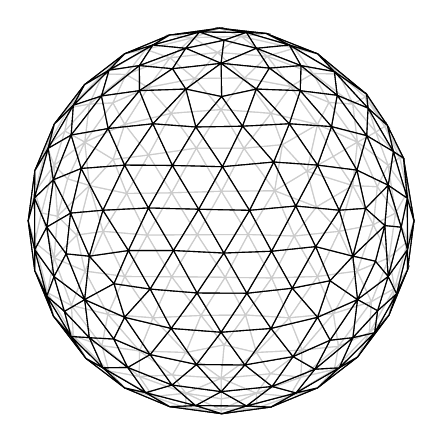
\begin{tikzpicture}[x={(1.732cm,-1cm)},y={(1.732cm,1cm)},z={(0,2cm)}]
\coordinate (v0) at (1.0,0.0,0.0);
\coordinate (v1) at (0.0,1.0,0.0);
\coordinate (v2) at (-1.0,0.0,0.0);
\coordinate (v3) at (0.0,-1.0,0.0);
\coordinate (v4) at (0.0,0.0,-1.0);
\coordinate (v5) at (0.0,0.0,1.0);
\coordinate (v6) at (0.9659258261113405,0.2588190457658098,0.0);
\coordinate (v7) at (0.8660254030594872,0.5000000012556528,0.0);
\coordinate (v8) at (0.7071067795767626,0.7071067827963324,0.0);
\coordinate (v9) at (0.4999999986418108,0.8660254045685896,0.0);
\coordinate (v10) at (0.2588190443111854,0.9659258265011059,0.0);
\coordinate (v11) at (-0.2588190457837957,0.9659258261065212,0.0);
\coordinate (v12) at (-0.5000000013601116,0.8660254029991779,0.0);
\coordinate (v13) at (-0.7071067828732788,0.7071067794998164,0.0);
\coordinate (v14) at (-0.8660254045816592,0.4999999986191735,0.0);
\coordinate (v15) at (-0.9659258264965713,0.258819044328109,0.0);
\coordinate (v16) at (-0.9659258261113405,-0.2588190457658098,0.0);
\coordinate (v17) at (-0.8660254030594872,-0.5000000012556528,0.0);
\coordinate (v18) at (-0.7071067795767626,-0.7071067827963324,0.0);
\coordinate (v19) at (-0.4999999986418108,-0.8660254045685896,0.0);
\coordinate (v20) at (-0.2588190443111854,-0.9659258265011059,0.0);
\coordinate (v21) at (0.2588190457837957,-0.9659258261065212,0.0);
\coordinate (v22) at (0.5000000013601116,-0.8660254029991779,0.0);
\coordinate (v23) at (0.7071067828732788,-0.7071067794998164,0.0);
\coordinate (v24) at (0.8660254045816592,-0.4999999986191735,0.0);
\coordinate (v25) at (0.9659258264965713,-0.258819044328109,0.0);
\coordinate (v26) at (0.0,0.9659258261113405,-0.2588190457658098);
\coordinate (v27) at (0.0,0.8660254030594872,-0.5000000012556528);
\coordinate (v28) at (0.0,0.7071067795767626,-0.7071067827963324);
\coordinate (v29) at (0.0,0.4999999986418108,-0.8660254045685896);
\coordinate (v30) at (0.0,0.2588190443111854,-0.9659258265011059);
\coordinate (v31) at (0.0,-0.2588190457837957,-0.9659258261065212);
\coordinate (v32) at (0.0,-0.5000000013601116,-0.8660254029991779);
\coordinate (v33) at (0.0,-0.7071067828732788,-0.7071067794998164);
\coordinate (v34) at (0.0,-0.8660254045816592,-0.4999999986191735);
\coordinate (v35) at (0.0,-0.9659258264965713,-0.258819044328109);
\coordinate (v36) at (0.0,-0.9659258261113405,0.2588190457658098);
\coordinate (v37) at (0.0,-0.8660254030594872,0.5000000012556528);
\coordinate (v38) at (0.0,-0.7071067795767626,0.7071067827963324);
\coordinate (v39) at (0.0,-0.4999999986418108,0.8660254045685896);
\coordinate (v40) at (0.0,-0.2588190443111854,0.9659258265011059);
\coordinate (v41) at (0.0,0.2588190457837957,0.9659258261065212);
\coordinate (v42) at (0.0,0.5000000013601116,0.8660254029991779);
\coordinate (v43) at (0.0,0.7071067828732788,0.7071067794998164);
\coordinate (v44) at (0.0,0.8660254045816592,0.4999999986191735);
\coordinate (v45) at (0.0,0.9659258264965713,0.258819044328109);
\coordinate (v46) at (0.9659258261113405,0.0,0.2588190457658098);
\coordinate (v47) at (0.8660254030594872,0.0,0.5000000012556528);
\coordinate (v48) at (0.7071067795767626,0.0,0.7071067827963324);
\coordinate (v49) at (0.4999999986418108,0.0,0.8660254045685896);
\coordinate (v50) at (0.2588190443111854,0.0,0.9659258265011059);
\coordinate (v51) at (-0.2588190457837957,0.0,0.9659258261065212);
\coordinate (v52) at (-0.5000000013601116,0.0,0.8660254029991779);
\coordinate (v53) at (-0.7071067828732788,0.0,0.7071067794998164);
\coordinate (v54) at (-0.8660254045816592,0.0,0.4999999986191735);
\coordinate (v55) at (-0.9659258264965713,0.0,0.258819044328109);
\coordinate (v56) at (-0.9659258261113405,0.0,-0.2588190457658098);
\coordinate (v57) at (-0.8660254030594872,0.0,-0.5000000012556528);
\coordinate (v58) at (-0.7071067795767626,0.0,-0.7071067827963324);
\coordinate (v59) at (-0.4999999986418108,0.0,-0.8660254045685896);
\coordinate (v60) at (-0.2588190443111854,0.0,-0.9659258265011059);
\coordinate (v61) at (0.2588190457837957,0.0,-0.9659258261065212);
\coordinate (v62) at (0.5000000013601116,0.0,-0.8660254029991779);
\coordinate (v63) at (0.7071067828732788,0.0,-0.7071067794998164);
\coordinate (v64) at (0.8660254045816592,0.0,-0.4999999986191735);
\coordinate (v65) at (0.9659258264965713,0.0,-0.258819044328109);
\coordinate (v66) at (-0.5968753305573024,0.7703416941999426,0.2243668893204343);
\coordinate (v67) at (-0.25808567630587,0.5868977891779429,0.7674443385243377);
\coordinate (v68) at (-0.7769544900097934,0.2245974601741118,0.5881537104468694);
\coordinate (v69) at (-0.2254249910932218,0.9001119381675856,0.3728385711795151);
\coordinate (v70) at (-0.3787640544764326,0.2205246094336313,0.8988508718213706);
\coordinate (v71) at (-0.9048480989796104,0.3705166486211054,0.2097429924492644);
\coordinate (v72) at (-0.7797560750556357,0.585705630718971,0.2212607189709846);
\coordinate (v73) at (-0.650709021142228,0.6242337603634365,0.4323440025673979);
\coordinate (v74) at (-0.4465168089496794,0.7845299651173139,0.4303022703153183);
\coordinate (v75) at (-0.231240816923478,0.7685299157113522,0.5965875924307369);
\coordinate (v76) at (-0.4739425155526548,0.6200993088613943,0.6251892743080067);
\coordinate (v77) at (-0.6031837146803123,0.2254193786783961,0.7651029255799586);
\coordinate (v78) at (-0.6513658012436212,0.442834451184977,0.6161415158185994);
\coordinate (v79) at (-0.8003871115687095,0.4251399784782245,0.422686045603888);
\coordinate (v80) at (-0.4439412469568365,0.4312895863375229,0.7854490254099811);
\coordinate (v81) at (-0.9039370819570685,0.20705058418685,0.3742357693408044);
\coordinate (v82) at (-0.3877851743099778,0.897240796860791,0.2112038465190635);
\coordinate (v83) at (-0.207731567320233,0.3928339621379274,0.895853933880903);
\coordinate (v84) at (-0.1761804132919844,0.9677027834328927,0.1803386000228983);
\coordinate (v85) at (-0.1685588971098267,0.1898373709799256,0.9672434916327717);
\coordinate (v86) at (-0.9684447980774777,0.1746040072380701,0.1778708464271154);
\coordinate (v87) at (-0.5968753307481794,-0.2243668895376927,0.7703416939887752);
\coordinate (v88) at (-0.2580856747343077,-0.76744433963247,0.5868977884200106);
\coordinate (v89) at (-0.7769544878960637,-0.5881537128406362,0.2245974612176846);
\coordinate (v90) at (-0.2254249911044945,-0.3728385711823959,0.9001119381635698);
\coordinate (v91) at (-0.3787640522362001,-0.89885087303886,0.2205246083185127);
\coordinate (v92) at (-0.904848098645285,-0.2097429941003022,0.3705166485031911);
\coordinate (v93) at (-0.779756075329191,-0.2212607195851551,0.585705630122805);
\coordinate (v94) at (-0.6507090211826841,-0.4323440022848056,0.6242337605170156);
\coordinate (v95) at (-0.4465168096565718,-0.4303022694920272,0.7845299651665554);
\coordinate (v96) at (-0.2312408167647887,-0.5965875924847092,0.7685299157171981);
\coordinate (v97) at (-0.4739425151141017,-0.6251892745748621,0.6200993089275739);
\coordinate (v98) at (-0.6031837130612882,-0.7651029268255582,0.2254193787829455);
\coordinate (v99) at (-0.6513658007101506,-0.6161415159905272,0.4428344517303621);
\coordinate (v100) at (-0.8003871102786878,-0.4226860477315288,0.4251399787912912);
\coordinate (v101) at (-0.4439412449754755,-0.7854490267443461,0.431289585947156);
\coordinate (v102) at (-0.9039370812790738,-0.3742357716630582,0.2070505829492741);
\coordinate (v103) at (-0.3877851738453488,-0.2112038471434982,0.8972407969146465);
\coordinate (v104) at (-0.2077315675057009,-0.8958539340303733,0.3928339616989984);
\coordinate (v105) at (-0.1761804137572365,-0.1803386002115927,0.9677027833130498);
\coordinate (v106) at (-0.1685588964450716,-0.9672434918215602,0.1898373706080592);
\coordinate (v107) at (-0.9684447978110251,-0.1778708478837493,0.1746040072323722);
\coordinate (v108) at (0.2373906267115964,0.5927409723817137,0.7696306924730116);
\coordinate (v109) at (0.7697707710048625,0.5952202488744707,0.2306363113500065);
\coordinate (v110) at (0.7715181150161288,0.2241412011263674,0.5954389220805305);
\coordinate (v111) at (0.2851758031801919,0.9150830133715486,0.2851758031775501);
\coordinate (v112) at (0.3692155676783176,0.2111788235332098,0.905046009811243);
\coordinate (v113) at (0.9150830123989893,0.2851758047394409,0.2851758047394476);
\coordinate (v114) at (0.2753900042236253,0.7911269310737263,0.546175264334329);
\coordinate (v115) at (0.5461752643497462,0.7911269310564869,0.2753900042425727);
\coordinate (v116) at (0.4619648243177169,0.6151122925083028,0.6389312148648023);
\coordinate (v117) at (0.641521731118863,0.6210132027869703,0.4503349340187716);
\coordinate (v118) at (0.8053380981320204,0.4199759472986743,0.4184238142857654);
\coordinate (v119) at (0.5855986155063985,0.2238194347714397,0.7791060214201453);
\coordinate (v120) at (0.63364096670642,0.433732440129488,0.6406140643019629);
\coordinate (v121) at (0.4273171617143365,0.423891712063688,0.7985878884122581);
\coordinate (v122) at (0.2100486925880666,0.3754812074457851,0.9027283031774649);
\coordinate (v123) at (0.4723957159889963,0.7465951543384605,0.4684612272726617);
\coordinate (v124) at (0.1756874204939024,0.1784127050819355,0.9681492048495346);
\coordinate (v125) at (0.8840112368180318,0.1746408047174856,0.4336434724045649);
\coordinate (v126) at (0.8794805302343316,0.4408052756453442,0.1795199461504336);
\coordinate (v127) at (0.9758097728955429,0.1559726491244944,0.1532147208624068);
\coordinate (v128) at (0.1593794995713874,0.9747557310275753,0.1563866823416694);
\coordinate (v129) at (0.1697430886237962,0.8877436557132312,0.4279248189208922);
\coordinate (v130) at (0.4162253125924886,0.8949040748362558,0.1610058480091539);
\coordinate (v131) at (-0.7723547397298042,0.229839038321006,-0.5921735093468681);
\coordinate (v132) at (-0.2319544372565306,0.7681237290935419,-0.5968336483317315);
\coordinate (v133) at (-0.6002447844336112,0.7681146429678114,-0.2230089224107618);
\coordinate (v134) at (-0.3728385711823655,0.2254249911044676,-0.9001119381635893);
\coordinate (v135) at (-0.9029228878282824,0.370193644323789,-0.2184322608026444);
\coordinate (v136) at (-0.2851758047477622,0.9150830123929419,-0.285175804750534);
\coordinate (v137) at (-0.5951954520500858,0.2326861098415221,-0.7691728827103976);
\coordinate (v138) at (-0.4173579798734024,0.4472140676990436,-0.7910989718946118);
\coordinate (v139) at (-0.7741596912071872,0.593014447795586,-0.2214441399507367);
\coordinate (v140) at (-0.6320078110726355,0.634393429350531,-0.4451075820328241);
\coordinate (v141) at (-0.4145091360595434,0.8075628348742852,-0.419586096516264);
\coordinate (v142) at (-0.2232586774497229,0.594825618287681,-0.7722467202843186);
\coordinate (v143) at (-0.442027272315798,0.6402729051141058,-0.6282297000268782);
\coordinate (v144) at (-0.901036262032701,0.2082665060571496,-0.3805044601932027);
\coordinate (v145) at (-0.7924702203401054,0.4297451505211725,-0.432823142783372);
\coordinate (v146) at (-0.6295156876644074,0.4543634859921001,-0.6302954482419656);
\coordinate (v147) at (-0.2096366631826169,0.3885403959646253,-0.8972815223758099);
\coordinate (v148) at (-0.9675893252358235,0.1758101501409081,-0.1813062535139228);
\coordinate (v149) at (-0.1680732355016323,0.1901950459158499,-0.967257730977304);
\coordinate (v150) at (-0.4336434737700136,0.8840112359203006,-0.1746408058717195);
\coordinate (v151) at (-0.1795199467464361,0.8794805300870903,-0.4408052756964803);
\coordinate (v152) at (-0.1532147209534412,0.9758097728748019,-0.1559726491648589);
\coordinate (v153) at (0.7657229958867138,0.6013042679501603,-0.2283168825477369);
\coordinate (v154) at (0.5877361365262779,0.2433726647591427,-0.7715982068018842);
\coordinate (v155) at (0.2254250129109098,0.7729438626059109,-0.5931006882585448);
\coordinate (v156) at (0.2176133561645956,0.3768755103605308,-0.9003527756399743);
\coordinate (v157) at (0.9001119381675905,0.2254249910932214,-0.3728385711795036);
\coordinate (v158) at (0.3787932747739996,0.901003975299685,-0.2115011355874853);
\coordinate (v159) at (0.5970339286614769,0.7725015625867129,-0.2163755122369979);
\coordinate (v160) at (0.6296043507869505,0.6434769922698669,-0.4353695214622952);
\coordinate (v161) at (0.768534062862255,0.2316585676444229,-0.5964201733242775);
\coordinate (v162) at (0.778859096757814,0.4518873813342889,-0.4349711884265977);
\coordinate (v163) at (0.6247354038022158,0.4619833128771551,-0.6295115010417719);
\coordinate (v164) at (0.23011863963793,0.5938356425391235,-0.770994116454625);
\coordinate (v165) at (0.4539570255996985,0.6487224386308964,-0.610811776273649);
\coordinate (v166) at (0.4347529553598408,0.4265616777137352,-0.7931336139907178);
\coordinate (v167) at (0.8964021109005491,0.3901819199384114,-0.2103491058737358);
\coordinate (v168) at (0.2128691406017332,0.9041562549852469,-0.3704231790863897);
\coordinate (v169) at (0.3853300004172362,0.2002884393565442,-0.9007938010718928);
\coordinate (v170) at (0.4335697012091362,0.798906198245832,-0.4168849084349718);
\coordinate (v171) at (0.1782009565922777,0.9677655603522645,-0.1780012466421906);
\coordinate (v172) at (0.9677538119750918,0.1795483917067467,-0.1767063714688659);
\coordinate (v173) at (0.1861291197390319,0.1763154172173644,-0.9665813403316981);
\coordinate (v174) at (-0.7704943006792206,-0.59710982040261,-0.2232158618824846);
\coordinate (v175) at (-0.2287168084391019,-0.5942629460650517,-0.771081962482446);
\coordinate (v176) at (-0.7729438626060494,-0.225425012911137,-0.5931006882582779);
\coordinate (v177) at (-0.3752955595818615,-0.901719900955972,-0.2146623967663249);
\coordinate (v178) at (-0.372838571182401,-0.225424991104492,-0.9001119381635685);
\coordinate (v179) at (-0.9150830123990066,-0.2851758047394184,-0.2851758047394148);
\coordinate (v180) at (-0.2151766899186381,-0.7754770001747973,-0.5935999542172238);
\coordinate (v181) at (-0.4368242221604006,-0.6471083226696589,-0.624856926085817);
\coordinate (v182) at (-0.4302556048369856,-0.4440037382365219,-0.7859806576517545);
\coordinate (v183) at (-0.5916150920544347,-0.239218380891727,-0.7699310318190187);
\coordinate (v184) at (-0.6308909327668567,-0.467733352975124,-0.619038883742423);
\coordinate (v185) at (-0.614587983026649,-0.6583496721760371,-0.4345901167994557);
\coordinate (v186) at (-0.8003097539065411,-0.4244380019930233,-0.4235371190648015);
\coordinate (v187) at (-0.4301369881804004,-0.7985152788615917,-0.4211677476646139);
\coordinate (v188) at (-0.5898880121883503,-0.776309387782573,-0.2222674340304155);
\coordinate (v189) at (-0.207731568497199,-0.3928339599670561,-0.8958539345599623);
\coordinate (v190) at (-0.1945517472087195,-0.9048553530467243,-0.3786946864308662);
\coordinate (v191) at (-0.1665780690137853,-0.1906387578805186,-0.9674289659956561);
\coordinate (v192) at (-0.1829409767921664,-0.9659672615242203,-0.1828955625390885);
\coordinate (v193) at (-0.8840112364740983,-0.4336434729242771,-0.1746408051681598);
\coordinate (v194) at (-0.8794805301669909,-0.1795199464211402,-0.4408052756694942);
\coordinate (v195) at (-0.9777920893726778,-0.1482194832423213,-0.1481882527629938);
\coordinate (v196) at (0.5951141306623251,-0.771360998253499,0.2255403394742468);
\coordinate (v197) at (0.2381722620478427,-0.5946827086731585,0.7678893295261325);
\coordinate (v198) at (0.7729438626064933,-0.2254250129110194,0.5931006882577443);
\coordinate (v199) at (0.9006206293770568,-0.3792903710026838,0.2122419166035303);
\coordinate (v200) at (0.2216723266252707,-0.9010051593762881,0.3729306002560798);
\coordinate (v201) at (0.377385998800413,-0.2201314083408526,0.8995265939060715);
\coordinate (v202) at (0.7772952789028376,-0.5882493438695642,0.2231630972496919);
\coordinate (v203) at (0.6474011490719067,-0.6270641183472476,0.4332130496658635);
\coordinate (v204) at (0.440977913386104,-0.7894918225741926,0.426926817450477);
\coordinate (v205) at (0.2402400413445714,-0.772542691726231,0.5877841768107366);
\coordinate (v206) at (0.4661174811643206,-0.6298251331439748,0.6213388486980316);
\coordinate (v207) at (0.595225348782834,-0.2097679201944678,0.7757127801797813);
\coordinate (v208) at (0.6521231806588578,-0.4440157397006633,0.6144879067302715);
\coordinate (v209) at (0.7989720496143149,-0.4292442929488189,0.421212320174436);
\coordinate (v210) at (0.4447569681669115,-0.4345957936598091,0.7831615818717098);
\coordinate (v211) at (0.8983430246080711,-0.205350738490668,0.3883757159412087);
\coordinate (v212) at (0.3812201894375025,-0.9008125066074991,0.2079252372165344);
\coordinate (v213) at (0.2077315664595707,-0.3928339595673662,0.8958539352075814);
\coordinate (v214) at (0.1823438369838656,-0.9673803970286905,0.1758870196407169);
\coordinate (v215) at (0.1805379416169278,-0.1767900139325556,0.9675544582965597);
\coordinate (v216) at (0.9675706945928364,-0.168717838984903,0.1880197601956982);
\coordinate (v217) at (0.5921735102805579,-0.7723547387630713,-0.2298390391640635);
\coordinate (v218) at (0.5968336480630774,-0.2319544371327693,-0.7681237293396584);
\coordinate (v219) at (0.2230089222143883,-0.600244784428311,-0.7681146430289603);
\coordinate (v220) at (0.9001119381676049,-0.3728385711794845,-0.2254249910931948);
\coordinate (v221) at (0.2184322608156712,-0.9029228876954322,-0.3701936446401466);
\coordinate (v222) at (0.2851758047588487,-0.2851758047588553,-0.915083012386894);
\coordinate (v223) at (0.76917288303696,-0.5951954515395242,-0.2326861100680429);
\coordinate (v224) at (0.7910989719184124,-0.4173579809643789,-0.4472140666387888);
\coordinate (v225) at (0.7722467196839322,-0.2232586794706518,-0.5948256183087112);
\coordinate (v226) at (0.2214441399410167,-0.7741596911311408,-0.5930144478984903);
\coordinate (v227) at (0.4451075823207684,-0.6320078102297472,-0.634393429988193);
\coordinate (v228) at (0.4195860962526905,-0.4145091359583019,-0.807562835063212);
\coordinate (v229) at (0.6282296993668646,-0.4420272719032937,-0.6402729060465315);
\coordinate (v230) at (0.3805044610945562,-0.9010362615995603,-0.2082665062844167);
\coordinate (v231) at (0.4328231441734263,-0.7924702192301187,-0.4297451511678274);
\coordinate (v232) at (0.6302954480652208,-0.6295156872519587,-0.4543634868086169);
\coordinate (v233) at (0.8972815220942609,-0.2096366637355367,-0.3885403963165883);
\coordinate (v234) at (0.1813062540696644,-0.967589325093164,-0.1758101503530989);
\coordinate (v235) at (0.9672577307597976,-0.1680732363709023,-0.1901950462540888);
\coordinate (v236) at (0.1746408041726567,-0.4336434718144752,-0.884011237215081);
\coordinate (v237) at (0.4408052757569241,-0.1795199468247579,-0.8794805300408145);
\coordinate (v238) at (0.1559726507051513,-0.1532147206022448,-0.9758097726837831);
\draw[fill=white, fill opacity=0.8] (v143) -- (v146) -- (v140) -- cycle;
\draw[fill=white, fill opacity=0.8] (v140) -- (v146) -- (v145) -- cycle;
\draw[fill=white, fill opacity=0.8] (v138) -- (v146) -- (v143) -- cycle;
\draw[fill=white, fill opacity=0.8] (v141) -- (v143) -- (v140) -- cycle;
\draw[fill=white, fill opacity=0.8] (v137) -- (v146) -- (v138) -- cycle;
\draw[fill=white, fill opacity=0.8] (v145) -- (v146) -- (v131) -- cycle;
\draw[fill=white, fill opacity=0.8] (v138) -- (v143) -- (v142) -- cycle;
\draw[fill=white, fill opacity=0.8] (v140) -- (v145) -- (v139) -- cycle;
\draw[fill=white, fill opacity=0.8] (v132) -- (v143) -- (v141) -- cycle;
\draw[fill=white, fill opacity=0.8] (v133) -- (v141) -- (v140) -- cycle;
\draw[fill=white, fill opacity=0.8] (v131) -- (v146) -- (v137) -- cycle;
\draw[fill=white, fill opacity=0.8] (v142) -- (v143) -- (v132) -- cycle;
\draw[fill=white, fill opacity=0.8] (v133) -- (v140) -- (v139) -- cycle;
\draw[fill=white, fill opacity=0.8] (v137) -- (v138) -- (v134) -- cycle;
\draw[fill=white, fill opacity=0.8] (v142) -- (v147) -- (v138) -- cycle;
\draw[fill=white, fill opacity=0.8] (v144) -- (v145) -- (v131) -- cycle;
\draw[fill=white, fill opacity=0.8] (v141) -- (v151) -- (v132) -- cycle;
\draw[fill=white, fill opacity=0.8] (v139) -- (v145) -- (v135) -- cycle;
\draw[fill=white, fill opacity=0.8] (v133) -- (v150) -- (v141) -- cycle;
\draw[fill=white, fill opacity=0.8] (v138) -- (v147) -- (v134) -- cycle;
\draw[fill=white, fill opacity=0.8] (v135) -- (v145) -- (v144) -- cycle;
\draw[fill=white, fill opacity=0.8] (v136) -- (v151) -- (v141) -- cycle;
\draw[fill=white, fill opacity=0.8] (v141) -- (v150) -- (v136) -- cycle;
\draw[fill=white, fill opacity=0.8] (v131) -- (v137) -- (v58) -- cycle;
\draw[fill=white, fill opacity=0.8] (v28) -- (v142) -- (v132) -- cycle;
\draw[fill=white, fill opacity=0.8] (v133) -- (v139) -- (v13) -- cycle;
\draw[fill=white, fill opacity=0.8] (v132) -- (v151) -- (v27) -- cycle;
\draw[fill=white, fill opacity=0.8] (v59) -- (v137) -- (v134) -- cycle;
\draw[fill=white, fill opacity=0.8] (v29) -- (v147) -- (v142) -- cycle;
\draw[fill=white, fill opacity=0.8] (v57) -- (v144) -- (v131) -- cycle;
\draw[fill=white, fill opacity=0.8] (v12) -- (v150) -- (v133) -- cycle;
\draw[fill=white, fill opacity=0.8] (v14) -- (v139) -- (v135) -- cycle;
\draw[fill=white, fill opacity=0.8] (v58) -- (v137) -- (v59) -- cycle;
\draw[fill=white, fill opacity=0.8] (v28) -- (v132) -- (v27) -- cycle;
\draw[fill=white, fill opacity=0.8] (v57) -- (v131) -- (v58) -- cycle;
\draw[fill=white, fill opacity=0.8] (v12) -- (v133) -- (v13) -- cycle;
\draw[fill=white, fill opacity=0.8] (v29) -- (v142) -- (v28) -- cycle;
\draw[fill=white, fill opacity=0.8] (v13) -- (v139) -- (v14) -- cycle;
\draw[fill=white, fill opacity=0.8] (v147) -- (v149) -- (v134) -- cycle;
\draw[fill=white, fill opacity=0.8] (v144) -- (v148) -- (v135) -- cycle;
\draw[fill=white, fill opacity=0.8] (v26) -- (v151) -- (v136) -- cycle;
\draw[fill=white, fill opacity=0.8] (v136) -- (v150) -- (v11) -- cycle;
\draw[fill=white, fill opacity=0.8] (v27) -- (v151) -- (v26) -- cycle;
\draw[fill=white, fill opacity=0.8] (v59) -- (v134) -- (v60) -- cycle;
\draw[fill=white, fill opacity=0.8] (v30) -- (v147) -- (v29) -- cycle;
\draw[fill=white, fill opacity=0.8] (v11) -- (v150) -- (v12) -- cycle;
\draw[fill=white, fill opacity=0.8] (v14) -- (v135) -- (v15) -- cycle;
\draw[fill=white, fill opacity=0.8] (v56) -- (v144) -- (v57) -- cycle;
\draw[fill=white, fill opacity=0.8] (v134) -- (v149) -- (v60) -- cycle;
\draw[fill=white, fill opacity=0.8] (v30) -- (v149) -- (v147) -- cycle;
\draw[fill=white, fill opacity=0.8] (v135) -- (v148) -- (v15) -- cycle;
\draw[fill=white, fill opacity=0.8] (v56) -- (v148) -- (v144) -- cycle;
\draw[fill=white, fill opacity=0.8] (v11) -- (v152) -- (v136) -- cycle;
\draw[fill=white, fill opacity=0.8] (v136) -- (v152) -- (v26) -- cycle;
\draw[fill=white, fill opacity=0.8] (v14) -- (v72) -- (v13) -- cycle;
\draw[fill=white, fill opacity=0.8] (v13) -- (v66) -- (v12) -- cycle;
\draw[fill=white, fill opacity=0.8] (v27) -- (v155) -- (v28) -- cycle;
\draw[fill=white, fill opacity=0.8] (v58) -- (v176) -- (v57) -- cycle;
\draw[fill=white, fill opacity=0.8] (v28) -- (v164) -- (v29) -- cycle;
\draw[fill=white, fill opacity=0.8] (v59) -- (v183) -- (v58) -- cycle;
\draw[fill=white, fill opacity=0.8] (v57) -- (v194) -- (v56) -- cycle;
\draw[fill=white, fill opacity=0.8] (v13) -- (v72) -- (v66) -- cycle;
\draw[fill=white, fill opacity=0.8] (v155) -- (v164) -- (v28) -- cycle;
\draw[fill=white, fill opacity=0.8] (v58) -- (v183) -- (v176) -- cycle;
\draw[fill=white, fill opacity=0.8] (v12) -- (v82) -- (v11) -- cycle;
\draw[fill=white, fill opacity=0.8] (v15) -- (v71) -- (v14) -- cycle;
\draw[fill=white, fill opacity=0.8] (v26) -- (v168) -- (v27) -- cycle;
\draw[fill=white, fill opacity=0.8] (v29) -- (v156) -- (v30) -- cycle;
\draw[fill=white, fill opacity=0.8] (v176) -- (v194) -- (v57) -- cycle;
\draw[fill=white, fill opacity=0.8] (v60) -- (v178) -- (v59) -- cycle;
\draw[fill=white, fill opacity=0.8] (v66) -- (v82) -- (v12) -- cycle;
\draw[fill=white, fill opacity=0.8] (v71) -- (v72) -- (v14) -- cycle;
\draw[fill=white, fill opacity=0.8] (v27) -- (v168) -- (v155) -- cycle;
\draw[fill=white, fill opacity=0.8] (v29) -- (v164) -- (v156) -- cycle;
\draw[fill=white, fill opacity=0.8] (v4) -- (v149) -- (v30) -- cycle;
\draw[fill=white, fill opacity=0.8] (v60) -- (v149) -- (v4) -- cycle;
\draw[fill=white, fill opacity=0.8] (v2) -- (v148) -- (v56) -- cycle;
\draw[fill=white, fill opacity=0.8] (v15) -- (v148) -- (v2) -- cycle;
\draw[fill=white, fill opacity=0.8] (v178) -- (v183) -- (v59) -- cycle;
\draw[fill=white, fill opacity=0.8] (v1) -- (v152) -- (v11) -- cycle;
\draw[fill=white, fill opacity=0.8] (v26) -- (v152) -- (v1) -- cycle;
\draw[fill=white, fill opacity=0.8] (v56) -- (v194) -- (v179) -- cycle;
\draw[fill=white, fill opacity=0.8] (v82) -- (v84) -- (v11) -- cycle;
\draw[fill=white, fill opacity=0.8] (v15) -- (v86) -- (v71) -- cycle;
\draw[fill=white, fill opacity=0.8] (v26) -- (v171) -- (v168) -- cycle;
\draw[fill=white, fill opacity=0.8] (v156) -- (v173) -- (v30) -- cycle;
\draw[fill=white, fill opacity=0.8] (v60) -- (v191) -- (v178) -- cycle;
\draw[fill=white, fill opacity=0.8] (v56) -- (v195) -- (v2) -- cycle;
\draw[fill=white, fill opacity=0.8] (v1) -- (v171) -- (v26) -- cycle;
\draw[fill=white, fill opacity=0.8] (v2) -- (v86) -- (v15) -- cycle;
\draw[fill=white, fill opacity=0.8] (v11) -- (v84) -- (v1) -- cycle;
\draw[fill=white, fill opacity=0.8] (v30) -- (v173) -- (v4) -- cycle;
\draw[fill=white, fill opacity=0.8] (v4) -- (v191) -- (v60) -- cycle;
\draw[fill=white, fill opacity=0.8] (v72) -- (v73) -- (v66) -- cycle;
\draw[fill=white, fill opacity=0.8] (v179) -- (v195) -- (v56) -- cycle;
\draw[fill=white, fill opacity=0.8] (v155) -- (v165) -- (v164) -- cycle;
\draw[fill=white, fill opacity=0.8] (v186) -- (v194) -- (v176) -- cycle;
\draw[fill=white, fill opacity=0.8] (v183) -- (v184) -- (v176) -- cycle;
\draw[fill=white, fill opacity=0.8] (v74) -- (v82) -- (v66) -- cycle;
\draw[fill=white, fill opacity=0.8] (v71) -- (v79) -- (v72) -- cycle;
\draw[fill=white, fill opacity=0.8] (v168) -- (v170) -- (v155) -- cycle;
\draw[fill=white, fill opacity=0.8] (v164) -- (v166) -- (v156) -- cycle;
\draw[fill=white, fill opacity=0.8] (v182) -- (v183) -- (v178) -- cycle;
\draw[fill=white, fill opacity=0.8] (v179) -- (v194) -- (v186) -- cycle;
\draw[fill=white, fill opacity=0.8] (v69) -- (v84) -- (v82) -- cycle;
\draw[fill=white, fill opacity=0.8] (v72) -- (v79) -- (v73) -- cycle;
\draw[fill=white, fill opacity=0.8] (v73) -- (v74) -- (v66) -- cycle;
\draw[fill=white, fill opacity=0.8] (v71) -- (v86) -- (v81) -- cycle;
\draw[fill=white, fill opacity=0.8] (v168) -- (v171) -- (v158) -- cycle;
\draw[fill=white, fill opacity=0.8] (v169) -- (v173) -- (v156) -- cycle;
\draw[fill=white, fill opacity=0.8] (v155) -- (v170) -- (v165) -- cycle;
\draw[fill=white, fill opacity=0.8] (v165) -- (v166) -- (v164) -- cycle;
\draw[fill=white, fill opacity=0.8] (v184) -- (v186) -- (v176) -- cycle;
\draw[fill=white, fill opacity=0.8] (v178) -- (v191) -- (v189) -- cycle;
\draw[fill=white, fill opacity=0.8] (v2) -- (v195) -- (v16) -- cycle;
\draw[fill=white, fill opacity=0.8] (v182) -- (v184) -- (v183) -- cycle;
\draw[fill=white, fill opacity=0.8] (v10) -- (v171) -- (v1) -- cycle;
\draw[fill=white, fill opacity=0.8] (v55) -- (v86) -- (v2) -- cycle;
\draw[fill=white, fill opacity=0.8] (v1) -- (v84) -- (v45) -- cycle;
\draw[fill=white, fill opacity=0.8] (v4) -- (v173) -- (v61) -- cycle;
\draw[fill=white, fill opacity=0.8] (v31) -- (v191) -- (v4) -- cycle;
\draw[fill=white, fill opacity=0.8] (v69) -- (v82) -- (v74) -- cycle;
\draw[fill=white, fill opacity=0.8] (v71) -- (v81) -- (v79) -- cycle;
\draw[fill=white, fill opacity=0.8] (v16) -- (v195) -- (v179) -- cycle;
\draw[fill=white, fill opacity=0.8] (v158) -- (v170) -- (v168) -- cycle;
\draw[fill=white, fill opacity=0.8] (v166) -- (v169) -- (v156) -- cycle;
\draw[fill=white, fill opacity=0.8] (v178) -- (v189) -- (v182) -- cycle;
\draw[fill=white, fill opacity=0.8] (v45) -- (v84) -- (v69) -- cycle;
\draw[fill=white, fill opacity=0.8] (v81) -- (v86) -- (v55) -- cycle;
\draw[fill=white, fill opacity=0.8] (v158) -- (v171) -- (v10) -- cycle;
\draw[fill=white, fill opacity=0.8] (v61) -- (v173) -- (v169) -- cycle;
\draw[fill=white, fill opacity=0.8] (v61) -- (v238) -- (v4) -- cycle;
\draw[fill=white, fill opacity=0.8] (v4) -- (v238) -- (v31) -- cycle;
\draw[fill=white, fill opacity=0.8] (v1) -- (v128) -- (v10) -- cycle;
\draw[fill=white, fill opacity=0.8] (v45) -- (v128) -- (v1) -- cycle;
\draw[fill=white, fill opacity=0.8] (v189) -- (v191) -- (v31) -- cycle;
\draw[fill=white, fill opacity=0.8] (v186) -- (v193) -- (v179) -- cycle;
\draw[fill=white, fill opacity=0.8] (v2) -- (v107) -- (v55) -- cycle;
\draw[fill=white, fill opacity=0.8] (v16) -- (v107) -- (v2) -- cycle;
\draw[fill=white, fill opacity=0.8] (v179) -- (v193) -- (v16) -- cycle;
\draw[fill=white, fill opacity=0.8] (v73) -- (v79) -- (v78) -- cycle;
\draw[fill=white, fill opacity=0.8] (v73) -- (v76) -- (v74) -- cycle;
\draw[fill=white, fill opacity=0.8] (v163) -- (v166) -- (v165) -- cycle;
\draw[fill=white, fill opacity=0.8] (v165) -- (v170) -- (v160) -- cycle;
\draw[fill=white, fill opacity=0.8] (v185) -- (v186) -- (v184) -- cycle;
\draw[fill=white, fill opacity=0.8] (v181) -- (v184) -- (v182) -- cycle;
\draw[fill=white, fill opacity=0.8] (v74) -- (v75) -- (v69) -- cycle;
\draw[fill=white, fill opacity=0.8] (v79) -- (v81) -- (v68) -- cycle;
\draw[fill=white, fill opacity=0.8] (v154) -- (v169) -- (v166) -- cycle;
\draw[fill=white, fill opacity=0.8] (v159) -- (v170) -- (v158) -- cycle;
\draw[fill=white, fill opacity=0.8] (v182) -- (v189) -- (v175) -- cycle;
\draw[fill=white, fill opacity=0.8] (v45) -- (v69) -- (v44) -- cycle;
\draw[fill=white, fill opacity=0.8] (v174) -- (v193) -- (v186) -- cycle;
\draw[fill=white, fill opacity=0.8] (v54) -- (v81) -- (v55) -- cycle;
\draw[fill=white, fill opacity=0.8] (v9) -- (v158) -- (v10) -- cycle;
\draw[fill=white, fill opacity=0.8] (v73) -- (v78) -- (v76) -- cycle;
\draw[fill=white, fill opacity=0.8] (v61) -- (v169) -- (v62) -- cycle;
\draw[fill=white, fill opacity=0.8] (v32) -- (v189) -- (v31) -- cycle;
\draw[fill=white, fill opacity=0.8] (v163) -- (v165) -- (v160) -- cycle;
\draw[fill=white, fill opacity=0.8] (v31) -- (v238) -- (v222) -- cycle;
\draw[fill=white, fill opacity=0.8] (v222) -- (v238) -- (v61) -- cycle;
\draw[fill=white, fill opacity=0.8] (v16) -- (v193) -- (v17) -- cycle;
\draw[fill=white, fill opacity=0.8] (v78) -- (v79) -- (v68) -- cycle;
\draw[fill=white, fill opacity=0.8] (v128) -- (v130) -- (v10) -- cycle;
\draw[fill=white, fill opacity=0.8] (v154) -- (v166) -- (v163) -- cycle;
\draw[fill=white, fill opacity=0.8] (v74) -- (v76) -- (v75) -- cycle;
\draw[fill=white, fill opacity=0.8] (v45) -- (v129) -- (v128) -- cycle;
\draw[fill=white, fill opacity=0.8] (v55) -- (v107) -- (v92) -- cycle;
\draw[fill=white, fill opacity=0.8] (v102) -- (v107) -- (v16) -- cycle;
\draw[fill=white, fill opacity=0.8] (v160) -- (v170) -- (v159) -- cycle;
\draw[fill=white, fill opacity=0.8] (v181) -- (v182) -- (v175) -- cycle;
\draw[fill=white, fill opacity=0.8] (v181) -- (v185) -- (v184) -- cycle;
\draw[fill=white, fill opacity=0.8] (v174) -- (v186) -- (v185) -- cycle;
\draw[fill=white, fill opacity=0.8] (v69) -- (v75) -- (v44) -- cycle;
\draw[fill=white, fill opacity=0.8] (v68) -- (v81) -- (v54) -- cycle;
\draw[fill=white, fill opacity=0.8] (v62) -- (v169) -- (v154) -- cycle;
\draw[fill=white, fill opacity=0.8] (v9) -- (v159) -- (v158) -- cycle;
\draw[fill=white, fill opacity=0.8] (v175) -- (v189) -- (v32) -- cycle;
\draw[fill=white, fill opacity=0.8] (v55) -- (v92) -- (v54) -- cycle;
\draw[fill=white, fill opacity=0.8] (v17) -- (v102) -- (v16) -- cycle;
\draw[fill=white, fill opacity=0.8] (v10) -- (v130) -- (v9) -- cycle;
\draw[fill=white, fill opacity=0.8] (v17) -- (v193) -- (v174) -- cycle;
\draw[fill=white, fill opacity=0.8] (v44) -- (v129) -- (v45) -- cycle;
\draw[fill=white, fill opacity=0.8] (v31) -- (v236) -- (v32) -- cycle;
\draw[fill=white, fill opacity=0.8] (v62) -- (v237) -- (v61) -- cycle;
\draw[fill=white, fill opacity=0.8] (v222) -- (v236) -- (v31) -- cycle;
\draw[fill=white, fill opacity=0.8] (v111) -- (v130) -- (v128) -- cycle;
\draw[fill=white, fill opacity=0.8] (v61) -- (v237) -- (v222) -- cycle;
\draw[fill=white, fill opacity=0.8] (v128) -- (v129) -- (v111) -- cycle;
\draw[fill=white, fill opacity=0.8] (v92) -- (v107) -- (v102) -- cycle;
\draw[fill=white, fill opacity=0.8] (v78) -- (v80) -- (v76) -- cycle;
\draw[fill=white, fill opacity=0.8] (v162) -- (v163) -- (v160) -- cycle;
\draw[fill=white, fill opacity=0.8] (v77) -- (v78) -- (v68) -- cycle;
\draw[fill=white, fill opacity=0.8] (v154) -- (v163) -- (v161) -- cycle;
\draw[fill=white, fill opacity=0.8] (v75) -- (v76) -- (v67) -- cycle;
\draw[fill=white, fill opacity=0.8] (v153) -- (v160) -- (v159) -- cycle;
\draw[fill=white, fill opacity=0.8] (v181) -- (v187) -- (v185) -- cycle;
\draw[fill=white, fill opacity=0.8] (v180) -- (v181) -- (v175) -- cycle;
\draw[fill=white, fill opacity=0.8] (v185) -- (v188) -- (v174) -- cycle;
\draw[fill=white, fill opacity=0.8] (v62) -- (v154) -- (v63) -- cycle;
\draw[fill=white, fill opacity=0.8] (v53) -- (v68) -- (v54) -- cycle;
\draw[fill=white, fill opacity=0.8] (v33) -- (v175) -- (v32) -- cycle;
\draw[fill=white, fill opacity=0.8] (v44) -- (v75) -- (v43) -- cycle;
\draw[fill=white, fill opacity=0.8] (v17) -- (v174) -- (v18) -- cycle;
\draw[fill=white, fill opacity=0.8] (v8) -- (v159) -- (v9) -- cycle;
\draw[fill=white, fill opacity=0.8] (v92) -- (v93) -- (v54) -- cycle;
\draw[fill=white, fill opacity=0.8] (v9) -- (v130) -- (v115) -- cycle;
\draw[fill=white, fill opacity=0.8] (v89) -- (v102) -- (v17) -- cycle;
\draw[fill=white, fill opacity=0.8] (v76) -- (v80) -- (v67) -- cycle;
\draw[fill=white, fill opacity=0.8] (v161) -- (v163) -- (v162) -- cycle;
\draw[fill=white, fill opacity=0.8] (v115) -- (v130) -- (v111) -- cycle;
\draw[fill=white, fill opacity=0.8] (v77) -- (v80) -- (v78) -- cycle;
\draw[fill=white, fill opacity=0.8] (v114) -- (v129) -- (v44) -- cycle;
\draw[fill=white, fill opacity=0.8] (v153) -- (v162) -- (v160) -- cycle;
\draw[fill=white, fill opacity=0.8] (v111) -- (v129) -- (v114) -- cycle;
\draw[fill=white, fill opacity=0.8] (v92) -- (v102) -- (v100) -- cycle;
\draw[fill=white, fill opacity=0.8] (v228) -- (v236) -- (v222) -- cycle;
\draw[fill=white, fill opacity=0.8] (v32) -- (v236) -- (v219) -- cycle;
\draw[fill=white, fill opacity=0.8] (v222) -- (v237) -- (v228) -- cycle;
\draw[fill=white, fill opacity=0.8] (v218) -- (v237) -- (v62) -- cycle;
\draw[fill=white, fill opacity=0.8] (v180) -- (v187) -- (v181) -- cycle;
\draw[fill=white, fill opacity=0.8] (v154) -- (v161) -- (v63) -- cycle;
\draw[fill=white, fill opacity=0.8] (v43) -- (v75) -- (v67) -- cycle;
\draw[fill=white, fill opacity=0.8] (v187) -- (v188) -- (v185) -- cycle;
\draw[fill=white, fill opacity=0.8] (v53) -- (v77) -- (v68) -- cycle;
\draw[fill=white, fill opacity=0.8] (v153) -- (v159) -- (v8) -- cycle;
\draw[fill=white, fill opacity=0.8] (v33) -- (v180) -- (v175) -- cycle;
\draw[fill=white, fill opacity=0.8] (v174) -- (v188) -- (v18) -- cycle;
\draw[fill=white, fill opacity=0.8] (v54) -- (v93) -- (v53) -- cycle;
\draw[fill=white, fill opacity=0.8] (v43) -- (v114) -- (v44) -- cycle;
\draw[fill=white, fill opacity=0.8] (v9) -- (v115) -- (v8) -- cycle;
\draw[fill=white, fill opacity=0.8] (v18) -- (v89) -- (v17) -- cycle;
\draw[fill=white, fill opacity=0.8] (v32) -- (v219) -- (v33) -- cycle;
\draw[fill=white, fill opacity=0.8] (v63) -- (v218) -- (v62) -- cycle;
\draw[fill=white, fill opacity=0.8] (v92) -- (v100) -- (v93) -- cycle;
\draw[fill=white, fill opacity=0.8] (v100) -- (v102) -- (v89) -- cycle;
\draw[fill=white, fill opacity=0.8] (v219) -- (v236) -- (v228) -- cycle;
\draw[fill=white, fill opacity=0.8] (v228) -- (v237) -- (v218) -- cycle;
\draw[fill=white, fill opacity=0.8] (v114) -- (v123) -- (v111) -- cycle;
\draw[fill=white, fill opacity=0.8] (v111) -- (v123) -- (v115) -- cycle;
\draw[fill=white, fill opacity=0.8] (v153) -- (v167) -- (v162) -- cycle;
\draw[fill=white, fill opacity=0.8] (v80) -- (v83) -- (v67) -- cycle;
\draw[fill=white, fill opacity=0.8] (v161) -- (v162) -- (v157) -- cycle;
\draw[fill=white, fill opacity=0.8] (v70) -- (v80) -- (v77) -- cycle;
\draw[fill=white, fill opacity=0.8] (v177) -- (v188) -- (v187) -- cycle;
\draw[fill=white, fill opacity=0.8] (v180) -- (v190) -- (v187) -- cycle;
\draw[fill=white, fill opacity=0.8] (v43) -- (v67) -- (v42) -- cycle;
\draw[fill=white, fill opacity=0.8] (v7) -- (v153) -- (v8) -- cycle;
\draw[fill=white, fill opacity=0.8] (v52) -- (v77) -- (v53) -- cycle;
\draw[fill=white, fill opacity=0.8] (v63) -- (v161) -- (v64) -- cycle;
\draw[fill=white, fill opacity=0.8] (v18) -- (v188) -- (v19) -- cycle;
\draw[fill=white, fill opacity=0.8] (v34) -- (v180) -- (v33) -- cycle;
\draw[fill=white, fill opacity=0.8] (v18) -- (v98) -- (v89) -- cycle;
\draw[fill=white, fill opacity=0.8] (v53) -- (v93) -- (v87) -- cycle;
\draw[fill=white, fill opacity=0.8] (v8) -- (v115) -- (v109) -- cycle;
\draw[fill=white, fill opacity=0.8] (v108) -- (v114) -- (v43) -- cycle;
\draw[fill=white, fill opacity=0.8] (v219) -- (v226) -- (v33) -- cycle;
\draw[fill=white, fill opacity=0.8] (v63) -- (v225) -- (v218) -- cycle;
\draw[fill=white, fill opacity=0.8] (v93) -- (v100) -- (v94) -- cycle;
\draw[fill=white, fill opacity=0.8] (v162) -- (v167) -- (v157) -- cycle;
\draw[fill=white, fill opacity=0.8] (v99) -- (v100) -- (v89) -- cycle;
\draw[fill=white, fill opacity=0.8] (v70) -- (v83) -- (v80) -- cycle;
\draw[fill=white, fill opacity=0.8] (v218) -- (v229) -- (v228) -- cycle;
\draw[fill=white, fill opacity=0.8] (v219) -- (v228) -- (v227) -- cycle;
\draw[fill=white, fill opacity=0.8] (v67) -- (v83) -- (v42) -- cycle;
\draw[fill=white, fill opacity=0.8] (v187) -- (v190) -- (v177) -- cycle;
\draw[fill=white, fill opacity=0.8] (v7) -- (v167) -- (v153) -- cycle;
\draw[fill=white, fill opacity=0.8] (v70) -- (v77) -- (v52) -- cycle;
\draw[fill=white, fill opacity=0.8] (v64) -- (v161) -- (v157) -- cycle;
\draw[fill=white, fill opacity=0.8] (v19) -- (v188) -- (v177) -- cycle;
\draw[fill=white, fill opacity=0.8] (v34) -- (v190) -- (v180) -- cycle;
\draw[fill=white, fill opacity=0.8] (v115) -- (v123) -- (v117) -- cycle;
\draw[fill=white, fill opacity=0.8] (v116) -- (v123) -- (v114) -- cycle;
\draw[fill=white, fill opacity=0.8] (v19) -- (v98) -- (v18) -- cycle;
\draw[fill=white, fill opacity=0.8] (v53) -- (v87) -- (v52) -- cycle;
\draw[fill=white, fill opacity=0.8] (v64) -- (v225) -- (v63) -- cycle;
\draw[fill=white, fill opacity=0.8] (v33) -- (v226) -- (v34) -- cycle;
\draw[fill=white, fill opacity=0.8] (v8) -- (v109) -- (v7) -- cycle;
\draw[fill=white, fill opacity=0.8] (v42) -- (v108) -- (v43) -- cycle;
\draw[fill=white, fill opacity=0.8] (v98) -- (v99) -- (v89) -- cycle;
\draw[fill=white, fill opacity=0.8] (v93) -- (v94) -- (v87) -- cycle;
\draw[fill=white, fill opacity=0.8] (v94) -- (v100) -- (v99) -- cycle;
\draw[fill=white, fill opacity=0.8] (v225) -- (v229) -- (v218) -- cycle;
\draw[fill=white, fill opacity=0.8] (v228) -- (v229) -- (v227) -- cycle;
\draw[fill=white, fill opacity=0.8] (v219) -- (v227) -- (v226) -- cycle;
\draw[fill=white, fill opacity=0.8] (v115) -- (v117) -- (v109) -- cycle;
\draw[fill=white, fill opacity=0.8] (v108) -- (v116) -- (v114) -- cycle;
\draw[fill=white, fill opacity=0.8] (v117) -- (v123) -- (v116) -- cycle;
\draw[fill=white, fill opacity=0.8] (v70) -- (v85) -- (v83) -- cycle;
\draw[fill=white, fill opacity=0.8] (v167) -- (v172) -- (v157) -- cycle;
\draw[fill=white, fill opacity=0.8] (v190) -- (v192) -- (v177) -- cycle;
\draw[fill=white, fill opacity=0.8] (v42) -- (v83) -- (v41) -- cycle;
\draw[fill=white, fill opacity=0.8] (v6) -- (v167) -- (v7) -- cycle;
\draw[fill=white, fill opacity=0.8] (v51) -- (v70) -- (v52) -- cycle;
\draw[fill=white, fill opacity=0.8] (v64) -- (v157) -- (v65) -- cycle;
\draw[fill=white, fill opacity=0.8] (v19) -- (v177) -- (v20) -- cycle;
\draw[fill=white, fill opacity=0.8] (v109) -- (v126) -- (v7) -- cycle;
\draw[fill=white, fill opacity=0.8] (v35) -- (v190) -- (v34) -- cycle;
\draw[fill=white, fill opacity=0.8] (v87) -- (v103) -- (v52) -- cycle;
\draw[fill=white, fill opacity=0.8] (v64) -- (v233) -- (v225) -- cycle;
\draw[fill=white, fill opacity=0.8] (v91) -- (v98) -- (v19) -- cycle;
\draw[fill=white, fill opacity=0.8] (v42) -- (v122) -- (v108) -- cycle;
\draw[fill=white, fill opacity=0.8] (v34) -- (v226) -- (v221) -- cycle;
\draw[fill=white, fill opacity=0.8] (v98) -- (v101) -- (v99) -- cycle;
\draw[fill=white, fill opacity=0.8] (v94) -- (v95) -- (v87) -- cycle;
\draw[fill=white, fill opacity=0.8] (v94) -- (v99) -- (v97) -- cycle;
\draw[fill=white, fill opacity=0.8] (v224) -- (v229) -- (v225) -- cycle;
\draw[fill=white, fill opacity=0.8] (v83) -- (v85) -- (v41) -- cycle;
\draw[fill=white, fill opacity=0.8] (v6) -- (v172) -- (v167) -- cycle;
\draw[fill=white, fill opacity=0.8] (v51) -- (v85) -- (v70) -- cycle;
\draw[fill=white, fill opacity=0.8] (v177) -- (v192) -- (v20) -- cycle;
\draw[fill=white, fill opacity=0.8] (v157) -- (v172) -- (v65) -- cycle;
\draw[fill=white, fill opacity=0.8] (v35) -- (v192) -- (v190) -- cycle;
\draw[fill=white, fill opacity=0.8] (v227) -- (v231) -- (v226) -- cycle;
\draw[fill=white, fill opacity=0.8] (v229) -- (v232) -- (v227) -- cycle;
\draw[fill=white, fill opacity=0.8] (v117) -- (v118) -- (v109) -- cycle;
\draw[fill=white, fill opacity=0.8] (v7) -- (v126) -- (v6) -- cycle;
\draw[fill=white, fill opacity=0.8] (v108) -- (v121) -- (v116) -- cycle;
\draw[fill=white, fill opacity=0.8] (v65) -- (v233) -- (v64) -- cycle;
\draw[fill=white, fill opacity=0.8] (v52) -- (v103) -- (v51) -- cycle;
\draw[fill=white, fill opacity=0.8] (v116) -- (v120) -- (v117) -- cycle;
\draw[fill=white, fill opacity=0.8] (v41) -- (v122) -- (v42) -- cycle;
\draw[fill=white, fill opacity=0.8] (v20) -- (v91) -- (v19) -- cycle;
\draw[fill=white, fill opacity=0.8] (v34) -- (v221) -- (v35) -- cycle;
\draw[fill=white, fill opacity=0.8] (v118) -- (v126) -- (v109) -- cycle;
\draw[fill=white, fill opacity=0.8] (v225) -- (v233) -- (v224) -- cycle;
\draw[fill=white, fill opacity=0.8] (v95) -- (v103) -- (v87) -- cycle;
\draw[fill=white, fill opacity=0.8] (v91) -- (v101) -- (v98) -- cycle;
\draw[fill=white, fill opacity=0.8] (v94) -- (v97) -- (v95) -- cycle;
\draw[fill=white, fill opacity=0.8] (v226) -- (v231) -- (v221) -- cycle;
\draw[fill=white, fill opacity=0.8] (v99) -- (v101) -- (v97) -- cycle;
\draw[fill=white, fill opacity=0.8] (v108) -- (v122) -- (v121) -- cycle;
\draw[fill=white, fill opacity=0.8] (v224) -- (v232) -- (v229) -- cycle;
\draw[fill=white, fill opacity=0.8] (v227) -- (v232) -- (v231) -- cycle;
\draw[fill=white, fill opacity=0.8] (v117) -- (v120) -- (v118) -- cycle;
\draw[fill=white, fill opacity=0.8] (v116) -- (v121) -- (v120) -- cycle;
\draw[fill=white, fill opacity=0.8] (v6) -- (v126) -- (v113) -- cycle;
\draw[fill=white, fill opacity=0.8] (v3) -- (v192) -- (v35) -- cycle;
\draw[fill=white, fill opacity=0.8] (v20) -- (v192) -- (v3) -- cycle;
\draw[fill=white, fill opacity=0.8] (v5) -- (v85) -- (v51) -- cycle;
\draw[fill=white, fill opacity=0.8] (v41) -- (v85) -- (v5) -- cycle;
\draw[fill=white, fill opacity=0.8] (v0) -- (v172) -- (v6) -- cycle;
\draw[fill=white, fill opacity=0.8] (v65) -- (v172) -- (v0) -- cycle;
\draw[fill=white, fill opacity=0.8] (v113) -- (v126) -- (v118) -- cycle;
\draw[fill=white, fill opacity=0.8] (v65) -- (v235) -- (v233) -- cycle;
\draw[fill=white, fill opacity=0.8] (v103) -- (v105) -- (v51) -- cycle;
\draw[fill=white, fill opacity=0.8] (v41) -- (v124) -- (v122) -- cycle;
\draw[fill=white, fill opacity=0.8] (v221) -- (v234) -- (v35) -- cycle;
\draw[fill=white, fill opacity=0.8] (v20) -- (v106) -- (v91) -- cycle;
\draw[fill=white, fill opacity=0.8] (v224) -- (v233) -- (v220) -- cycle;
\draw[fill=white, fill opacity=0.8] (v90) -- (v103) -- (v95) -- cycle;
\draw[fill=white, fill opacity=0.8] (v91) -- (v104) -- (v101) -- cycle;
\draw[fill=white, fill opacity=0.8] (v113) -- (v127) -- (v6) -- cycle;
\draw[fill=white, fill opacity=0.8] (v121) -- (v122) -- (v112) -- cycle;
\draw[fill=white, fill opacity=0.8] (v221) -- (v231) -- (v230) -- cycle;
\draw[fill=white, fill opacity=0.8] (v97) -- (v101) -- (v88) -- cycle;
\draw[fill=white, fill opacity=0.8] (v0) -- (v235) -- (v65) -- cycle;
\draw[fill=white, fill opacity=0.8] (v5) -- (v124) -- (v41) -- cycle;
\draw[fill=white, fill opacity=0.8] (v95) -- (v97) -- (v96) -- cycle;
\draw[fill=white, fill opacity=0.8] (v51) -- (v105) -- (v5) -- cycle;
\draw[fill=white, fill opacity=0.8] (v6) -- (v127) -- (v0) -- cycle;
\draw[fill=white, fill opacity=0.8] (v35) -- (v234) -- (v3) -- cycle;
\draw[fill=white, fill opacity=0.8] (v3) -- (v106) -- (v20) -- cycle;
\draw[fill=white, fill opacity=0.8] (v223) -- (v232) -- (v224) -- cycle;
\draw[fill=white, fill opacity=0.8] (v233) -- (v235) -- (v220) -- cycle;
\draw[fill=white, fill opacity=0.8] (v231) -- (v232) -- (v217) -- cycle;
\draw[fill=white, fill opacity=0.8] (v90) -- (v105) -- (v103) -- cycle;
\draw[fill=white, fill opacity=0.8] (v122) -- (v124) -- (v112) -- cycle;
\draw[fill=white, fill opacity=0.8] (v120) -- (v121) -- (v119) -- cycle;
\draw[fill=white, fill opacity=0.8] (v118) -- (v120) -- (v110) -- cycle;
\draw[fill=white, fill opacity=0.8] (v230) -- (v234) -- (v221) -- cycle;
\draw[fill=white, fill opacity=0.8] (v91) -- (v106) -- (v104) -- cycle;
\draw[fill=white, fill opacity=0.8] (v118) -- (v125) -- (v113) -- cycle;
\draw[fill=white, fill opacity=0.8] (v223) -- (v224) -- (v220) -- cycle;
\draw[fill=white, fill opacity=0.8] (v95) -- (v96) -- (v90) -- cycle;
\draw[fill=white, fill opacity=0.8] (v101) -- (v104) -- (v88) -- cycle;
\draw[fill=white, fill opacity=0.8] (v96) -- (v97) -- (v88) -- cycle;
\draw[fill=white, fill opacity=0.8] (v230) -- (v231) -- (v217) -- cycle;
\draw[fill=white, fill opacity=0.8] (v119) -- (v121) -- (v112) -- cycle;
\draw[fill=white, fill opacity=0.8] (v217) -- (v232) -- (v223) -- cycle;
\draw[fill=white, fill opacity=0.8] (v110) -- (v125) -- (v118) -- cycle;
\draw[fill=white, fill opacity=0.8] (v46) -- (v127) -- (v113) -- cycle;
\draw[fill=white, fill opacity=0.8] (v110) -- (v120) -- (v119) -- cycle;
\draw[fill=white, fill opacity=0.8] (v25) -- (v235) -- (v0) -- cycle;
\draw[fill=white, fill opacity=0.8] (v50) -- (v124) -- (v5) -- cycle;
\draw[fill=white, fill opacity=0.8] (v5) -- (v105) -- (v40) -- cycle;
\draw[fill=white, fill opacity=0.8] (v0) -- (v127) -- (v46) -- cycle;
\draw[fill=white, fill opacity=0.8] (v3) -- (v234) -- (v21) -- cycle;
\draw[fill=white, fill opacity=0.8] (v36) -- (v106) -- (v3) -- cycle;
\draw[fill=white, fill opacity=0.8] (v220) -- (v235) -- (v25) -- cycle;
\draw[fill=white, fill opacity=0.8] (v40) -- (v105) -- (v90) -- cycle;
\draw[fill=white, fill opacity=0.8] (v112) -- (v124) -- (v50) -- cycle;
\draw[fill=white, fill opacity=0.8] (v21) -- (v234) -- (v230) -- cycle;
\draw[fill=white, fill opacity=0.8] (v113) -- (v125) -- (v46) -- cycle;
\draw[fill=white, fill opacity=0.8] (v104) -- (v106) -- (v36) -- cycle;
\draw[fill=white, fill opacity=0.8] (v88) -- (v104) -- (v37) -- cycle;
\draw[fill=white, fill opacity=0.8] (v24) -- (v223) -- (v220) -- cycle;
\draw[fill=white, fill opacity=0.8] (v90) -- (v96) -- (v39) -- cycle;
\draw[fill=white, fill opacity=0.8] (v0) -- (v216) -- (v25) -- cycle;
\draw[fill=white, fill opacity=0.8] (v46) -- (v216) -- (v0) -- cycle;
\draw[fill=white, fill opacity=0.8] (v5) -- (v215) -- (v50) -- cycle;
\draw[fill=white, fill opacity=0.8] (v40) -- (v215) -- (v5) -- cycle;
\draw[fill=white, fill opacity=0.8] (v3) -- (v214) -- (v36) -- cycle;
\draw[fill=white, fill opacity=0.8] (v21) -- (v214) -- (v3) -- cycle;
\draw[fill=white, fill opacity=0.8] (v49) -- (v119) -- (v112) -- cycle;
\draw[fill=white, fill opacity=0.8] (v22) -- (v230) -- (v217) -- cycle;
\draw[fill=white, fill opacity=0.8] (v40) -- (v90) -- (v39) -- cycle;
\draw[fill=white, fill opacity=0.8] (v24) -- (v220) -- (v25) -- cycle;
\draw[fill=white, fill opacity=0.8] (v38) -- (v96) -- (v88) -- cycle;
\draw[fill=white, fill opacity=0.8] (v47) -- (v125) -- (v110) -- cycle;
\draw[fill=white, fill opacity=0.8] (v49) -- (v112) -- (v50) -- cycle;
\draw[fill=white, fill opacity=0.8] (v21) -- (v230) -- (v22) -- cycle;
\draw[fill=white, fill opacity=0.8] (v37) -- (v104) -- (v36) -- cycle;
\draw[fill=white, fill opacity=0.8] (v217) -- (v223) -- (v23) -- cycle;
\draw[fill=white, fill opacity=0.8] (v110) -- (v119) -- (v48) -- cycle;
\draw[fill=white, fill opacity=0.8] (v46) -- (v125) -- (v47) -- cycle;
\draw[fill=white, fill opacity=0.8] (v38) -- (v88) -- (v37) -- cycle;
\draw[fill=white, fill opacity=0.8] (v23) -- (v223) -- (v24) -- cycle;
\draw[fill=white, fill opacity=0.8] (v39) -- (v96) -- (v38) -- cycle;
\draw[fill=white, fill opacity=0.8] (v22) -- (v217) -- (v23) -- cycle;
\draw[fill=white, fill opacity=0.8] (v48) -- (v119) -- (v49) -- cycle;
\draw[fill=white, fill opacity=0.8] (v47) -- (v110) -- (v48) -- cycle;
\draw[fill=white, fill opacity=0.8] (v212) -- (v214) -- (v21) -- cycle;
\draw[fill=white, fill opacity=0.8] (v211) -- (v216) -- (v46) -- cycle;
\draw[fill=white, fill opacity=0.8] (v25) -- (v216) -- (v199) -- cycle;
\draw[fill=white, fill opacity=0.8] (v36) -- (v214) -- (v200) -- cycle;
\draw[fill=white, fill opacity=0.8] (v213) -- (v215) -- (v40) -- cycle;
\draw[fill=white, fill opacity=0.8] (v50) -- (v215) -- (v201) -- cycle;
\draw[fill=white, fill opacity=0.8] (v22) -- (v212) -- (v21) -- cycle;
\draw[fill=white, fill opacity=0.8] (v47) -- (v211) -- (v46) -- cycle;
\draw[fill=white, fill opacity=0.8] (v25) -- (v199) -- (v24) -- cycle;
\draw[fill=white, fill opacity=0.8] (v36) -- (v200) -- (v37) -- cycle;
\draw[fill=white, fill opacity=0.8] (v39) -- (v213) -- (v40) -- cycle;
\draw[fill=white, fill opacity=0.8] (v50) -- (v201) -- (v49) -- cycle;
\draw[fill=white, fill opacity=0.8] (v199) -- (v216) -- (v211) -- cycle;
\draw[fill=white, fill opacity=0.8] (v200) -- (v214) -- (v212) -- cycle;
\draw[fill=white, fill opacity=0.8] (v201) -- (v215) -- (v213) -- cycle;
\draw[fill=white, fill opacity=0.8] (v49) -- (v207) -- (v48) -- cycle;
\draw[fill=white, fill opacity=0.8] (v24) -- (v202) -- (v23) -- cycle;
\draw[fill=white, fill opacity=0.8] (v48) -- (v198) -- (v47) -- cycle;
\draw[fill=white, fill opacity=0.8] (v23) -- (v196) -- (v22) -- cycle;
\draw[fill=white, fill opacity=0.8] (v37) -- (v205) -- (v38) -- cycle;
\draw[fill=white, fill opacity=0.8] (v38) -- (v197) -- (v39) -- cycle;
\draw[fill=white, fill opacity=0.8] (v201) -- (v207) -- (v49) -- cycle;
\draw[fill=white, fill opacity=0.8] (v199) -- (v202) -- (v24) -- cycle;
\draw[fill=white, fill opacity=0.8] (v196) -- (v212) -- (v22) -- cycle;
\draw[fill=white, fill opacity=0.8] (v198) -- (v211) -- (v47) -- cycle;
\draw[fill=white, fill opacity=0.8] (v200) -- (v205) -- (v37) -- cycle;
\draw[fill=white, fill opacity=0.8] (v197) -- (v213) -- (v39) -- cycle;
\draw[fill=white, fill opacity=0.8] (v48) -- (v207) -- (v198) -- cycle;
\draw[fill=white, fill opacity=0.8] (v23) -- (v202) -- (v196) -- cycle;
\draw[fill=white, fill opacity=0.8] (v38) -- (v205) -- (v197) -- cycle;
\draw[fill=white, fill opacity=0.8] (v199) -- (v211) -- (v209) -- cycle;
\draw[fill=white, fill opacity=0.8] (v200) -- (v212) -- (v204) -- cycle;
\draw[fill=white, fill opacity=0.8] (v201) -- (v213) -- (v210) -- cycle;
\draw[fill=white, fill opacity=0.8] (v199) -- (v209) -- (v202) -- cycle;
\draw[fill=white, fill opacity=0.8] (v209) -- (v211) -- (v198) -- cycle;
\draw[fill=white, fill opacity=0.8] (v204) -- (v212) -- (v196) -- cycle;
\draw[fill=white, fill opacity=0.8] (v201) -- (v210) -- (v207) -- cycle;
\draw[fill=white, fill opacity=0.8] (v204) -- (v205) -- (v200) -- cycle;
\draw[fill=white, fill opacity=0.8] (v210) -- (v213) -- (v197) -- cycle;
\draw[fill=white, fill opacity=0.8] (v207) -- (v208) -- (v198) -- cycle;
\draw[fill=white, fill opacity=0.8] (v202) -- (v203) -- (v196) -- cycle;
\draw[fill=white, fill opacity=0.8] (v205) -- (v206) -- (v197) -- cycle;
\draw[fill=white, fill opacity=0.8] (v202) -- (v209) -- (v203) -- cycle;
\draw[fill=white, fill opacity=0.8] (v208) -- (v209) -- (v198) -- cycle;
\draw[fill=white, fill opacity=0.8] (v207) -- (v210) -- (v208) -- cycle;
\draw[fill=white, fill opacity=0.8] (v203) -- (v204) -- (v196) -- cycle;
\draw[fill=white, fill opacity=0.8] (v204) -- (v206) -- (v205) -- cycle;
\draw[fill=white, fill opacity=0.8] (v206) -- (v210) -- (v197) -- cycle;
\draw[fill=white, fill opacity=0.8] (v203) -- (v209) -- (v208) -- cycle;
\draw[fill=white, fill opacity=0.8] (v203) -- (v206) -- (v204) -- cycle;
\draw[fill=white, fill opacity=0.8] (v208) -- (v210) -- (v206) -- cycle;
\draw[fill=white, fill opacity=0.8] (v203) -- (v208) -- (v206) -- cycle;
\end{tikzpicture}
  \caption{Discretisation of a sphere into flat surface triangles.}
  \label{fig:triangulation}
\end{figure}

The first step is the \textbf{discretisation of the surface} $\Gamma$. Surfaces are represented in Bempp-cl as a triangulation into flat triangles (see \cref{fig:triangulation}). The triangulation is internally represented as an array of node coordinates and an associated connectivity array of node indices that define each triangle. In this step, topology data is also computed: in particular, for each triangle, we compute the neighboring triangles and the type of intersection (i.e. are they connected by an edge or a vertex).

Once a triangulation is given we need to define the necessary data structures for the discretisation. Bempp-cl uses a Galerkin discretisation: we introduce set of basis functions \(\phi_1\) to \(\phi_N\), and define the \textbf{trial space} as the span of these function. We then approximate the solution \(\phi\) of \cref{eq:bnd_integral} by $\phi_h=\sum_{j=1}^N \dvec{x}_j\phi_j$, where $\dvec{x}$ is a vector of coefficients. In the most simple case, we can define the function \(\phi_j\) to be equal to 1 on the triangle $\tau_j$ and 0 everywhere else. Other spaces are commonly defined to be piecewise polynomials on each triangle.

To discretise \cref{eq:bnd_integral}, we define a \textbf{test (or dual) space} in terms of a basis \(\psi_1\) to \(\psi_N\). The discrete representation of the above problem then takes the form
$$
\dmat{A}\dvec{x} = \dvec{b}
$$
with
\begin{align*}
\dmat{A}_{ij} &= \int_{\Gamma}\psi_i(\bx)\int_{\Gamma}g(\bx, \by)\phi_j(\bx)\ds[\by]\ds[\bx]\\
\dvec{b}_i &= \int_{\Gamma}\psi_i(\bx)f(\bx)\ds[\bx].
\end{align*}
In the case of piecewise constant trial and test functions, the definition of $\dmat{A}_{ij}$ simplifies to $\dmat{A}_{ij} = \int_{\Gamma}\int_{\Gamma}g(\bx, \by)\ds[\by]\ds[\bx]$.

In Bempp-cl, an operator definition consists of the type of the operator (e.g. Laplace single-layer in the above example),
the definition of the trial and test spaces, and the definition of the range space. The range space is required for operator
products and not relevant for the purpose of this paper. The function $f$ is represented as a \textbf{grid function} object, which
consists of either the dual representation in the forms of the integrals $\dvec{b}_i = \int_{\Gamma}\psi_i(\bx)f(\bx)\ds[\bx]$ or directly through its coefficients $f_j$ in the representation $f=\sum_{j=1}^N f_j\phi_j$.

Once the grid, the space objects, and the operator(s) are defined, the main computational step is performed, namely the \textbf{computation of the discrete matrix entries} $\dmat{A}_{ij}$. For pairs of triangles $\tau_i$ and $\tau_j$ that do not share a joint edge or vertex this is done through a simple numerical quadrature rule that approximates $\dmat{A}_{ij}\approx \sum_{\ell}\sum_{q} g(\bx_\ell, \by_q)\psi_i(\bx_\ell)\phi_j(\by_q)\omega_\ell\omega_q$, where the $\bx_\ell$ and $\by_q$ are quadrature points in the corresponding triangles $\tau_i$ and $\tau_j$, and the values $\omega_i$ and $\omega_j$ are the quadrature weights. In the case that two triangles share a joint vertex/edge or the triangles $\tau_i$ and $\tau_j$ are identical, corresponding singularity adapted quadrature numerical quadrature rules are used that are based on singularity removing coordinate transformations.

The values $\dvec{b}_i$ of the right-hand side vector $b$ are similarly computed through a numerical quadrature rule.

In the final step, \textbf{Bempp solves the underlying linear system of equations} either through a direct LU decomposition or through iterative solvers such as GMRES. The solution can then be evaluated away from the surface $\Gamma$ through domain potential operators and exported in various formats for visualisation.

In summary, to solve a boundary integral equation problem, the following steps are performed by Bempp:
\begin{enumerate}
	\item Import of the surface description as triangulation data.
	\item Definition of the trial space, test space and range space.
	\item Discretisation into a matrix problem $\dmat{A}\dvec{x}=\dvec{b}$.
	\item Solution of the matrix problem by either a direct or iterative solver.
	\item Evaluation of domain potential operators for visualisation and post-processing.
\end{enumerate}

All of these steps are accelerated through the use of either Numba or OpenCL. In the following section we provide a high-level overview of the library and how these acceleration techniques are deployed before we deep dive into the design of the computational kernels.

\section{A high level overview of Bempp-cl}

\begin{figure}
	\centering
    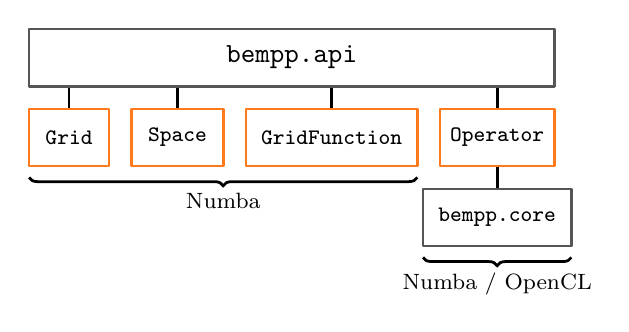
\begin{tikzpicture}[x=1.45cm,y=-1.45cm]

\draw[line width=1pt] (0.35,0.5) -- (0.35,0.7);
\draw[line width=1pt] (1.3,0.5) -- (1.3,0.7);
\draw[line width=1pt] (2.65,0.5) -- (2.65,0.7);
\draw[line width=1pt] (4.1,0.5) -- (4.1,0.7);
\draw[line width=1pt] (4.1,1.2) -- (4.1,1.4);

\draw[line width=1pt,line join=round,line cap=round,bemppgrey] (0,0) rectangle (4.6,0.5);
\node at (2.3,0.25) {\pyth{bempp.api}};
\draw[line width=1pt,line join=round,line cap=round,bempporange] (0,0.7) rectangle (0.7,1.2);
\node at (0.35,0.95) {\footnotesize \pyth{Grid}};
\draw[line width=1pt,line join=round,line cap=round,bempporange] (0.9,0.7) rectangle (1.7,1.2);
\node at (1.3,0.95) {\footnotesize \pyth{Space}};
\draw[line width=1pt,line join=round,line cap=round,bempporange] (1.9,0.7) rectangle (3.4,1.2);
\node at (2.65,0.95) {\footnotesize \pyth{GridFunction}};
\draw[line width=1pt,line join=round,line cap=round,bempporange] (3.6,0.7) rectangle (4.6,1.2);
\node at (4.1,0.95) {\footnotesize \pyth{Operator}};
\draw[line width=1pt,line join=round,line cap=round,bemppgrey] (3.45,1.4) rectangle (4.75,1.9);
\node at (4.1,1.65) {\footnotesize\pyth{bempp.core}};

\draw[line width=1pt,decorate,decoration={brace,amplitude=3pt,mirror}] (0,1.3) -- (3.4,1.3);
\node[anchor=north] at (1.7,1.35) {\footnotesize Numba};

\draw[line width=1pt,decorate,decoration={brace,amplitude=3pt,mirror}] (3.45,2) -- (4.75,2);
\node[anchor=north] at (4.1,2.05) {\footnotesize Numba / OpenCL};
\end{tikzpicture}

	\caption{The layout of Bempp-cl with its computational backends.}
	\label{fig:overview}
\end{figure}

The main user-visible component of Bempp-cl is the module \texttt{bempp.api}, which defines all user interface functions and other high-level routines. In particular, it contains the definition of the main object types: \texttt{Grid}, \texttt{Space}, \texttt{GridFunction}, \texttt{Operator}. All computational backend routines are part of \texttt{bempp.core}. We are currently supporting a full Numba backend and an OpenCL backend. An overview of this structure is provided in \cref{fig:overview}.

Outside the operator discretisation, Numba is used in the following contexts:
\begin{itemize}
	\item Topological computations for the grid. Finding out all neighbour relationships between triangles requires parses through the grid data structure with linear complexity, which is accelerated with Numba.
	\item Definition of local-to-global maps for function spaces. Again, this requires traversal through the grid and assigning relationships between global and local indices.
	\item Grid Functions. A right-hand side function $f$ can be defined as a Python callable. This is just-in-time compiled via Numba and then the product with the corresponding basis functions integrated in each triangle via numerical quadrature, again via Numba accelerated routines.
	\item Sparse matrices. Sparse surface matrices are assembled through Numba accelerated routines.
\end{itemize}

The main computational complexity in discretising the boundary integral equation \cref{eq:bnd_integral} is coming from the discretisation of the left-hand side integral operator. Using dense methods this has quadratic complexity in the number of surface triangles.

Once the user defines an operator with its associated discretisation spaces and calls the \textbf{weak\_form} method to discretize it the code calls a regular integrator to assemble all the interactions between non-adjacent elements and a singular integrator to compute the interactions between adjacent triangles (only necessary if trial and test space are defined on the same grid). The result is stored internally as a dense Numpy array. The corresponding discretisation routines are proxies that forward to computational routines in either Numba or OpenCL, depending on the user preferences. For OpenCL assembly the code checks additional parameters, such as the default vector length for SIMD operators (e.g. 4 for double precision and 8 for single precision in Intel AVX2, or 1 if a GPU is used), and whether the discretisation should proceed in single or double precision. The OpenCL kernel is then compiled for the underlying compute device using PyOpenCL and executed. If the computational backend is Numba, the call is forwarded to the corresponding Numba discretisation routines and executed. For simple piecewise constant function spaces or other spaces, where the support of each basis function is localized to a single triangle, only one call to the computational routines is necessary. If the support of basis functions is larger than a single triangle different threads may need to sum into the same global degree of freedom. We discuss this in more detail in \cref{sec:coloring}.

\section{Assembling boundary integral operators with OpenCL}

In this section we discuss in more detail the assembly of boundary integral operators with OpenCL
and how we integrated this into our Python workflow. We start with a brief introduction to OpenCL and then
dive into how we use OpenCL as part of Bempp-cl.

\subsection{What is OpenCL?}

OpenCL (\url{https://www.khronos.org/opencl/}) is a heterogeneous compute standard for CPUs, GPUs, FPGAs, and other types of devices that provide conformant drivers. At its core OpenCL executes compute kernels that can be written in C99, or more recently, in C++. The current version of OpenCL is 3.0, though the most widely implemented standard is OpenCL 1.2, which Bempp-cl uses. OpenCL splits the computational tasks into work-items, each of which represents a single execution of a compute kernel. Work items are grouped together into work-groups, which share local memory. Barrier synchronization is only allowed within a work-group. All work-items are uniquely indexed by a one, two, or three dimensional index space, called NDRange. Kernels are launched onto a compute device (e.g. CPU or GPU) from a host device. OpenCL allows kernels to be loaded as strings and compiled on the fly for a given device, making it well suited for launching from high-productivity languages. To launch an OpenCL kernel the following steps need to be performed.
\begin{itemize}
	\item Initialize buffers on the compute device.
	\item Compute relevant data from host to the compute device.
	\item Load a kernel string and just-in-time compile it for the device.
	\item Execute the kernel for the given buffers and chosen index space.
	\item Copy results back to the host.
\end{itemize}
An excellent feature of OpenCL is its very good support for vectorized operations. OpenCL provides vector data types, such as \textbf{double4}, that can hold four double values in a SIMD register and defines a number of standard operations for these vector types. This makes it easy to explicitly target modern SIMD execution in a portable way while avoiding difficult compiler intrinsics and keeping kernel code readable.

Python has excellent OpenCL support through the PyOpenCL library by Andreas Kloeckner, which automates much of the initialization of the OpenCL environment and makes it easy to create buffers and launch OpenCL kernels from Python.

\subsection{OpenCL Assembly in Bempp-cl}

\begin{figure*}
	\center
	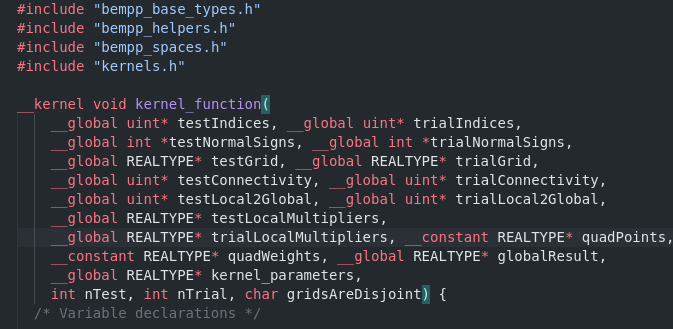
\includegraphics[width=12cm]{img/kernel_header}
	\caption{Definition of the OpenCL compute kernel for scalar integral equations.}
	\label{fig:kernel_definition}
\end{figure*}


Bempp-cl has OpenCL kernels for all its boundary operators. All operators have the same interface and are launched in the same way. In the first step the relevant data will need to be copied to the compute device. This data consists of:

\begin{itemize}
	\item Test and trial indices of triangles over which to be integrated.
	\item Signs of the normal directions for the spaces.
	\item Test and trial grid as flat floating point array, defining each triangle through nine floating point numbers, specifying the $(x, y, z)$ coordinates of each of the three nodes of a triangle.
	\item Test and trial connectivity information that stores the indices of each node for each triangle.
	\item Test and trial mappings of local triangle degrees of freedom to global degrees of freedom.
	\item Test and trial basis function multipliers for each triangle.
	\item Quadrature points and quadrature weights.
	\item A buffer that contains the global assembled matrix.
	\item Additional kernel parameters, such as the wavenumber for Helmholtz problems.
	\item Number of test and trial degrees of freedom.
	\item A single byte that is set to one if the test and trial grids are disjoint.
\end{itemize}
The actual kernel definition is shown in Figure \ref{fig:kernel_definition}.
Before the kernel can be launched, it needs to be configured and just-in-time compiled. Kernel configuration happens through C-style preprocessor definitions that are passed through the just-in-time compiler. These include the names of the test and trial space, the name of the function that evaluates the integral kernel, choosing between single and double precision types, and for SIMD enhanced kernel the vector length of the SIMD types.
For example, in Figure \ref{fig:kernel_definition} all floating point types have the name REALTYPE. This is substituted with either \textit{float} or \textit{double} during just-in-time compilation.

Each work-item computes via numerical quadrature all interactions via the integral kernel of basis functions on the trial element with basis functions on the test element. Before summing the result into the global result buffer, the kernel checks via the connectivity information if the test and trial triangle are adjoint or identical. For this it simply checks if at at least one of the node indices of the test triangle is identical to one of the node indices of the trial triangle. If this is true and the grids are not disjoint, the result of the kernel is discarded and not summed back into the global result buffer. The reason is that for adjoint triangles a separate singular quadrature rule is used. The effect is that a few work-items do work that is discarded. However, in a grid with $N$ elements the number of triangle pairs requiring a singular quadrature rule is $\mathcal{O}(N)$, while the total number of interactions is $N^2$. Hence, only a tiny fraction of work-items are discarded.


\subsection{SIMD optimized kernels}

The above description was valid for kernels that do not take advantage of CPU SIMD operations are kernels that run directly on a GPU device. For SIMD optimization on CPUs we proceed slightly differently. The corresponding kernel in principle works as described above, but batches together the interaction on one test triangle with X trial triangles, where X is either 4, 8, or 16, depending on the number of available SIMD lanes. This strategy allows us to optimize almost all floating point operations within a kernel run for SIMD operation. If the number of trial elements is not divisible by 4, 8, or 16, then the few remaining trial elements are assembled with the standard-non vectorized kernel.

Each kernel definition is stored in two variants, one with the ending \textit{\_novec.cl} and another one with the ending \textit{\_vec.cl}. The vectorized variant is configured via preprocessor directives for the desired number of vector lanes. Having to develop two OpenCL kernel codes for each operator is a certain amount of overhead. If we write a new kernel, we first implement the non-vectorized version. Then, with the help of preprocessor directives and a number of helper functions that do the actual implementation of operations depending on whether the kernel is vectorized or not, it is usually a matter of an hour or two to convert the non-vectorized kernel into a vectorized version.

Alternatively, some CPU OpenCL runtime environments have the option to try and auto-vectorize kernels by batching together work items on SIMD lanes, similarly to what we do manually. In our experience this works well for very simple kernels but often fails for more complex OpenCL kernels. This is why we decided to implement this strategy manually.

A completely different SIMD strategy is based on batching together quadrature evaluations within a single test/triangle pair. There are two disadvantages to this approach. First, it only works well if the number of quadrature points is a multiple of the available SIMD lanes. Second, other operations such as the geometry calculations for each element then can not be SIMD optimized as these are only performed once per test/triangle pair.


\subsection{Assembling the singular part of integral operators}

The assembly of the singular part of an integral operator works a bit differently. Remember that the singular part consists of triangle parts which are adjacent to each other or identical. There are $\mathcal{O}(N)$ of such pairs. We are using fully numerical quadrature rules for these integrals that are based on subdividing the four-dimensional integration domain and using transformation techniques to remove the singularities. This gives highly accurate evaluations of these integration pairs but requires a large number (typically over $1000$) quadrature points per triangle pair. Hence, we create one workgroup for each triangle pair and inside this workgroup have a number of work-items that are evaluating the quadrature rules and then at the end sum up the result together. Depending on how two triangles are in relationship to each other different types of singular quadrature rules are needed. We solve this pre-loading all possible quadrature rules onto the device and also store for each triangle pair an index into the required quadrature rule so that the kernel function can select the correct rule to evaluate. For the singular quadrature rules we did not implement separate SIMD optimized kernels as the proposed implementation is already highly efficient and requires only a fraction of the computational time of the regular quadrature rules described above. At the end, the singular integral values are either summed into the overall result matrix, or if desired by the user, stored as separate sparse matrix.

\section{Numba assembly of integral operators}

The Numba assembly of integral operators is structured differently from the OpenCL assembly. In OpenCL we create a large number of work-items that are executed in parallel on the compute device by the runtime system with the details of the parallel execution left to the device driver. For Numba we use classical loop based parallelism. Each loop iteration is the assembly of one test element with all trial elements. Within each loop we partially optimized for SIMD instruction, though this depends on the autovectorization of the just-in-time compiler and cannot be explicitly targeted in Numba. Again, we separate regular and singular interactions. In the next section we give some more details on SIMD optimization in Numba at the example of the Laplace kernel.

\section{SIMD optimized evaluation of the Laplace kernel with Numba}


\section{NUMBA ASSEMBLY OF INTEGRAL OPERATORS}
The main focus of Numba within Bempp-cl is to provide accelerated implementations of routines with linear complexity, such as grid iterations, integration of functions over grids, or assembly of certain sparse matrices. However, we also provide a fall-back implementation of the OpenCL dense operator assembly in Numba.

With Numba, we use loop parallelism: each loop iteration is the assembly of one test triangle with all trial triangles. We then parallelize over the test triangles through a parallel for-loop.
Within each loop we try to optimize for auto-vectorization by linearly passing through the data in memory order for the individual operations. However, a much smaller fraction of operations is SIMD optimized due to the lack of targeted SIMD constructs in Numba.

We stress that while Numba provides backends not only for CPU, but also for ROCm and CUDA, we currently only use the CPU component of Numba.

\section{PERFORMANCE BENCHMARKS}

In this section, we provide a number of performance benchmarks. The tests are running on a Dell Precision 7740 Workstation Laptop with 64 GB RAM. Its CPU is an Intel i9-9980HK with a base clock of 2.4GHz and a burst clock of 5GHz. The CPU supports AVX, AVX2, and AVX-512.
As a GPU we use an Nvidia Quadro RTX 3000 GPU. All benchmark tests were performed in Linux. For OpenCL on the GPU, we use the Nvidia GPU drivers and as CPU runtime we compare the open-source PoCL driver against the Intel CPU OpenCL runtime environment. All timing runs were repeated several times to make sure that the overhead from running the OpenCL and Numba JIT compilers did not skew the results. Though hardly noticeable by users, for smaller experiments the JIT phase typically takes longer than the actual computation.

\subsection{Dense Operator assembly}
We start by benchmarking the dense operator assembly. We assemble the matrix $\dmat{A}$ defined by
$$
\dmat{A}_{ij} = \int_{\Gamma}\psi_i(\bx)\int_{\Gamma}\frac{\phi_j(\by)}{4\uppi |\bx -\by|}\ds[\by]\ds[\bx],
$$
with $\Gamma$ being the unit sphere. For the basis functions $\phi_j$ and test functions $\psi_i$, we compare two cases: piecewise constant functions for both (P0 functions); and nodal, piecewise linear, and globally continuous functions for both (P1 functions). In the P0 case, each triangle is associated with just one piecewise constant function. In the P1 case, each triangle is associated with $3$ linear basis functions, one for each node of the triangle.

We first compare the OpenCL CPU performance for the Intel OpenCL runtime, and the PoCL OpenCL runtime driver. We run the tests in single precision and double precision. The native vector width for both drivers in single precision is $8$, and in double precision is $4$, which corresponds to AVX instructions. In Bempp-cl, this means that we assemble in vectorized form one test triangle with $8$ trial triangles in single precision, and with $4$ trial triangles in double precision. Within the assembly, almost all floating point instructions are manually vectorized to take advantage of this. We should hence see up a factor 2 speed-up between single and double precision assembly.

\begin{figure}
	\center
	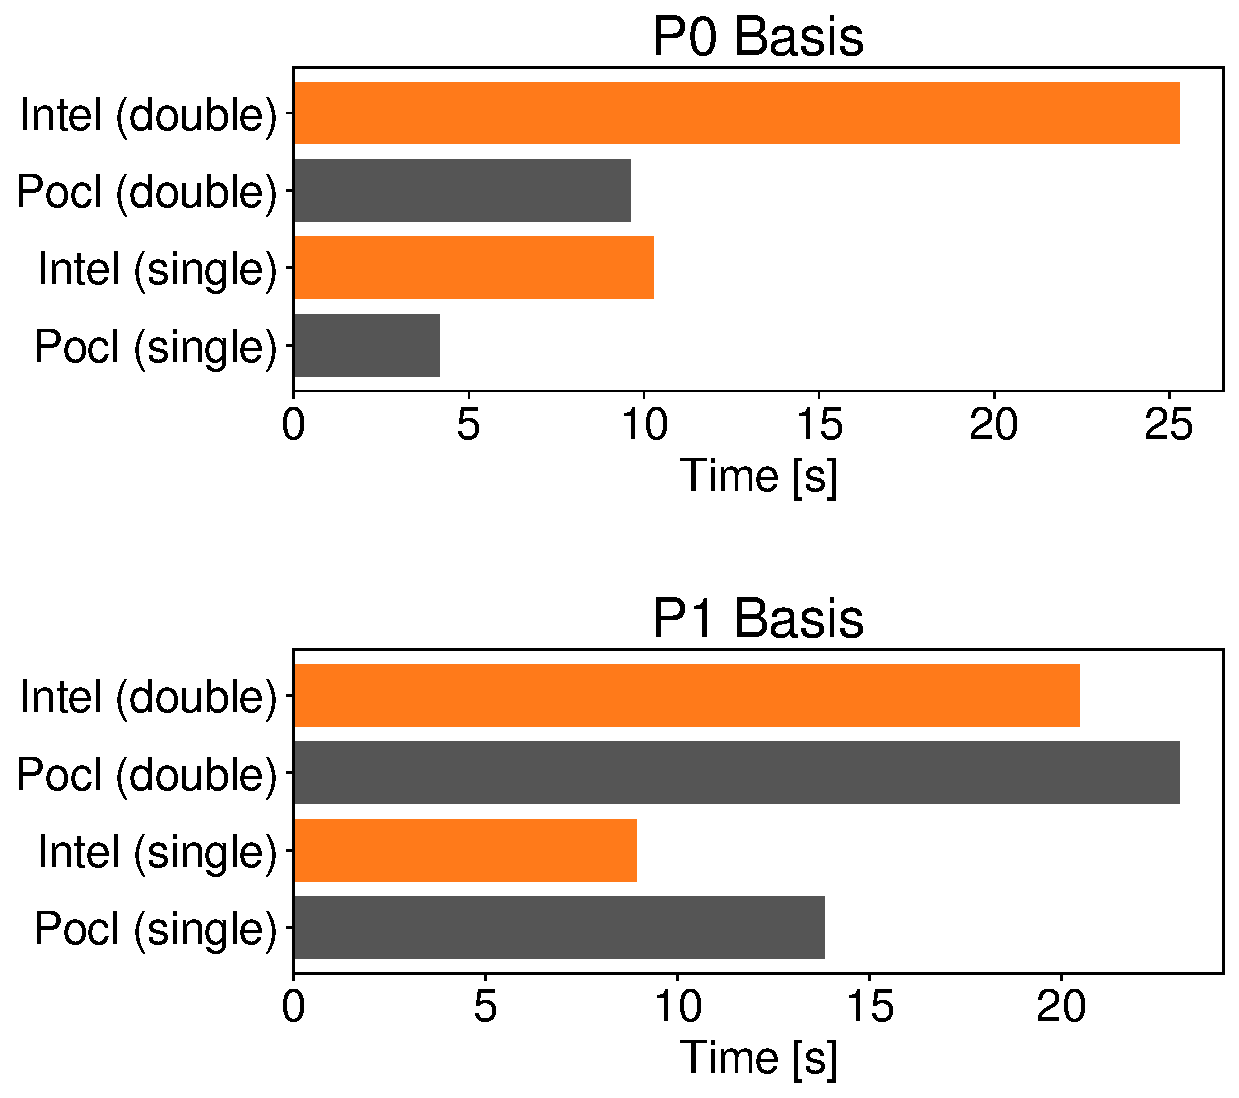
\includegraphics[width=6cm]{img/intel_pocl_laplace_comp.pdf}
	\caption{Comparison of the performance of PoCL and the Intel OpenCL runtime for the assembly of the Laplace single-layer boundary operator on a grid with 32,768 elements.}
	\label{fig:intel_pocl_laplace_cmp}
\end{figure}

The timings for a grid with 32,768 elements are shown in \cref{fig:intel_pocl_laplace_cmp}. We see the expected speed-up between single precision and double precision evaluation. It is interesting to note the difference between the Intel and the PoCL runtime environment. For P0 basis functions, the PoCL driver (gray bar) significantly outperforms the Intel driver (orange bar) in both single and double precision. For P1 basis functions, however, the Intel driver gives better performance.

In \cref{fig:pocl_single_layer}, we compare specifically the performance of single precision and double precision evaluation for the PoCL driver for various grid sizes in the case of a P0 basis. We can see that the speed-up for larger grid sizes is slightly more than just a factor of two. The final data point in this graph corresponds to the grid size used for \cref{fig:intel_pocl_laplace_cmp}.

\begin{figure}
	\center
	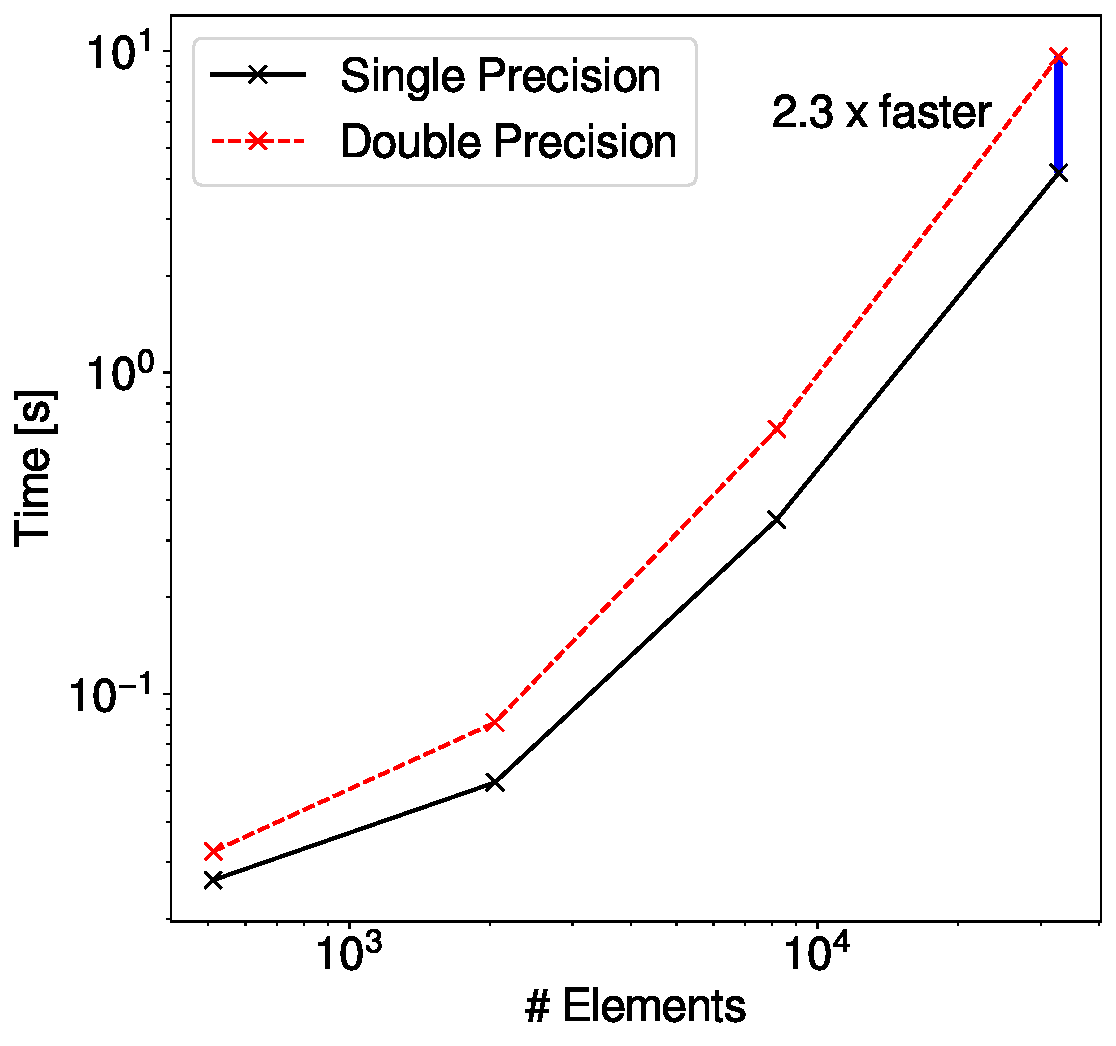
\includegraphics[width=7cm]{img/pocl_single_layer.pdf}
	\caption{Comparison of the single-precision and double-precision performance for various grid sizes using PoCL and P0 basis functions.}
	\label{fig:pocl_single_layer}
\end{figure}

\begin{figure}
\begin{center}
\begin{tabular}{l|c|c}
	        &   single      &    double\\
	        \hline
	 PoCL   &   0.05s       &    0.08s\\
	 Numba  &   0.25s       &    0.25s\\
	 GPU    &   0.11s       &    3.00s\\
\end{tabular}
\end{center}
\caption{Comparison of PoCL, Numba and GPU Assembly for a grid with 2048 elements.}
\label{fig:cpu_gpu_numba_compare}
\end{figure}
In Bempp-cl, we can easily switch between CPU Assembly, GPU Assembly, and Numba Assembly. \Cref{fig:cpu_gpu_numba_compare} shows a comparison between these modes for a grid with 2048 elements. The speed differences are striking. GPU assembly in single precision is a factor of two slower than CPU assembly (and much slower in double precision due to Nvidia hardware restrictions for double precision). Numba is five times slower for single precision and still around three times slower for double precision than PoCL. The GPU behaviour can be explained by data transfer: while the GPU kernels themselves are extremely fast, data transfer over the bus severely limits performance. Even for medium sized problems, we have to transfer the data back to the main memory as GPU RAM is too limited to keep dense matrices with a tens of thousands or rows and columns on the device.

An alternative method is to compute the matrix-vector product (matvec) $\dmat{A}\dvec{x}$ on the device without first computing the dense matrix $\dmat{A}$. This can be done by recomputing all matrix elements during each matvec calculation on-the-fly and not storing them. We have done experiments with this, and observed significant speed-ups compared to CPU evaluation as we now only need to transfer single vectors over the bus. For larger problems, however, it is not competitive compared to accelerated methods such as fast multipole methods (FMM), due to the quadratic complexity of direct evaluation of the matvec compared to linear complexity of FMM. For smaller problems, it is still practically better to just assemble the whole matrix and store it, as then matvecs are much faster for an iterative solver. Hence, we can conclude that there is only limited practical relevance for on-the-fly GPU evaluation of boundary integral operators. There are, however, very significant practical advantages of on-the-fly evaluation of the evaluation of domain potential operators for visualization and post-processing, as we will see in the next section.

The Numba performance difference seen in \cref{fig:cpu_gpu_numba_compare} is interesting. The main reason for this, we believe, is significantly lower usage of AVX vectorized instructions. We have taken care to optimize the Green's function evaluation for auto-vectorized evaluation in Numba, but the loops over integration points and other operations auto-vectorize very badly when just looping over all trial triangle for a single test triangle, as we currently do. We could tune our code for better auto-vectorization in Numba, but this would give little benefit as we have highly optimized hand-tuned OpenCL kernels already. We therefore recommend using Numba for operator assembly only as a fallback if no OpenCL runtime is available.

\subsection{Evaluating domain potentials for post-processing of electromagnetic problems}
Once an integral equation is solved, one is usually interested in evaluating the solution not only at the boundary but also at points away from it. To do this, we evaluate the integral
$$
f(\bx) = \int_{\Gamma}g(\bx, \by)\phi(\by) \ds[\by]
$$
for many points $\bx$ away from the boundary $\Gamma$. For example, if we want to visualize a solution, we take the points $\bx$ to be a regular grid of points.

Typically, we want to do only a small number of potential evaluations at the end of a calculation. Discretising this operation into a dense matrix and then evaluating the dense matrix-vector product is not practical for larger sizes. For very large problems with hundreds of thousands of elements, we use FMM or other accelerated approximate methods. For moderately sized problems with a few ten thousand elements up to around a hundred thousand elements (depending on the problem at hand), direct evaluation of this integral for every point $\bx$ is highly efficient. We won't go into the details of the corresponding OpenCL kernels here, but we show some results that demonstrate the relative performance on CPUs and GPUs.

For the dense assembly of boundary integral operators, the performance was limited by the bus transfer of the dense matrix. For the evaluation of domain potentials, however, we only need to transfer to the device the vector of coefficients of the basis functions for $\phi$, and then transfer back to the host the values at the points $\bx$.

In this section, we consider the evaluation of the electric potential operator, defined by
\begin{multline}
\left(\mathcal{E}\mathbf{p}\right)(\bx) = \ii k\int_{\Gamma}\mathbf{p}(\by)g(\bx, \by) \ds[\by]\\
-\frac{1}{\ii k}\nabla_{\bx}\int_{\Gamma}\operatorname{div}\mathbf{p}(\by)g(\bx, \by)\ds[\by],
\end{multline}
where $g(\bx, \by) = \frac{\ee^{\ii k|\bx - \by|}}{4\pi|\bx - \by|}$ is the Helmholtz Green's function, and
$k$ the wavenumber of the problem.
The function $\mathbf{p}:\mathbb{R}^3\to\mathbb{R}^3$ is a vector-valued function, leading to an overall vector solution at each point $\bx$. The implementation of electromagnetic problems in Bempp is covered in detail in \cite{bempp_maxwell}. For these experiments, we again use a grid with 32,768 elements and RWG (Rao, Wilton, and Glisson) edge-based basis functions. For the potential evaluation, we use 50,000 random evaluation points in the exterior of the unit sphere, and as wavenumber use $k=1.0$.

In \cref{fig:efield_domain_potential}, we compare the performance of GPU evaluation with that of the PoCL CPU driver. In single-precision, the GPU significantly outperforms the CPU; and even in double-precision, the Nvidia Quadro RTX GPU is faster than the 8-core CPU, even though its hardware is not optimised for fast double-precision operations.

\begin{figure}
	\center
	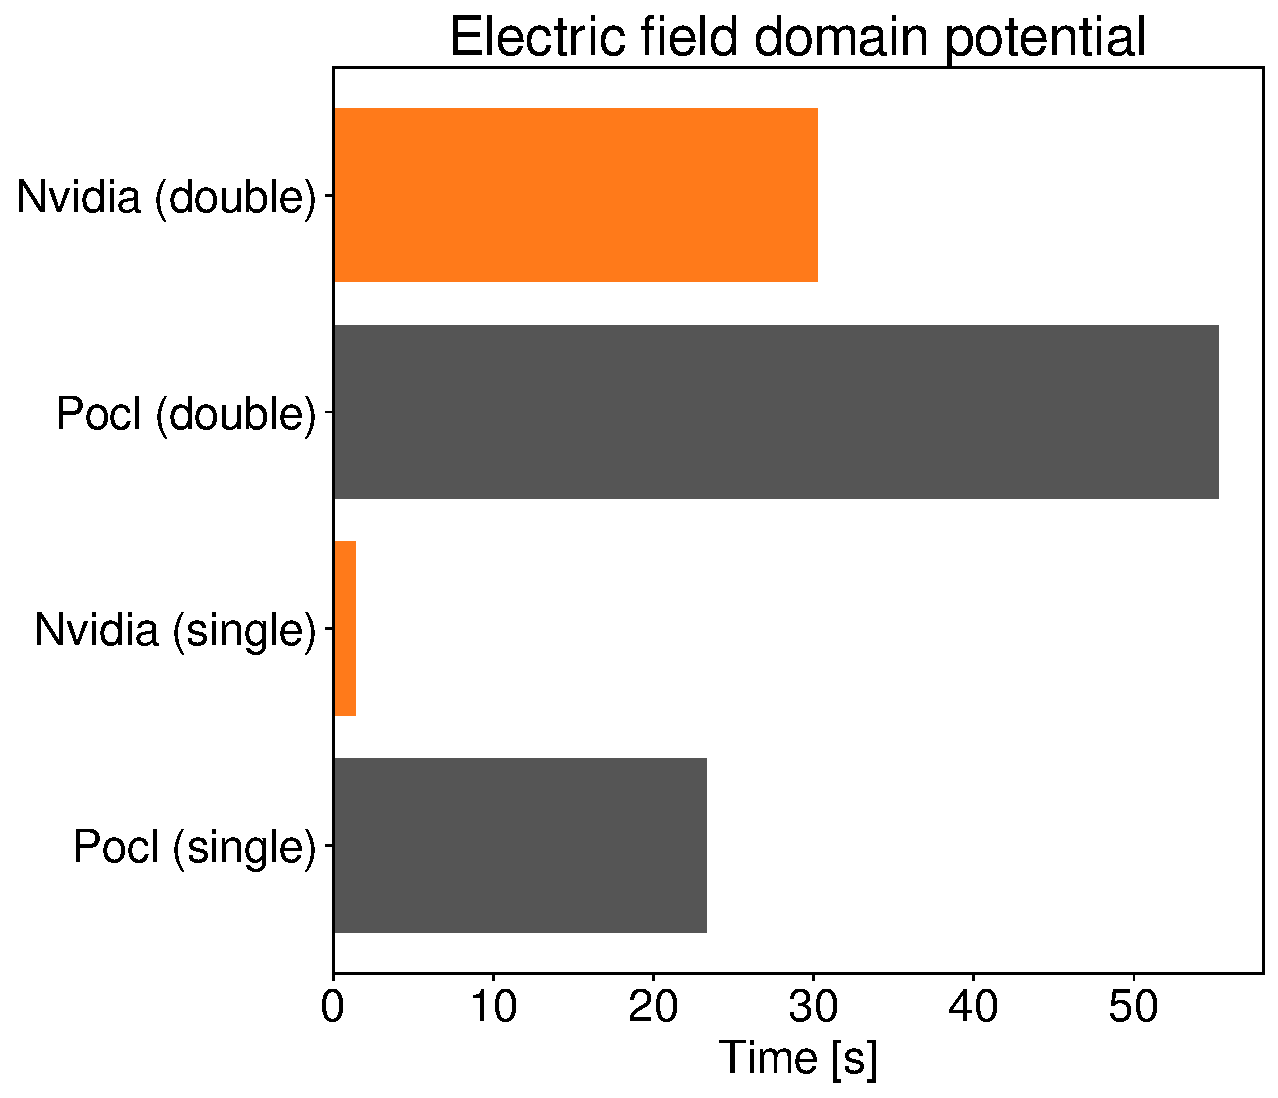
\includegraphics[width=7cm]{img/efield_domain_potential.pdf}
	\caption{Evaluation of an electric field potential operator on CPU via PoCL vs GPU}
	\label{fig:efield_domain_potential}
\end{figure}

\section{SUMMARY}
With Bempp-cl, we have created a Python library that achieves high-performance through use of modern just-in-time compilation technologies. Bempp-cl mixes Numba evaluation for less compute intensive linear complexity loops and sparse matrix generation with highly optimized OpenCL kernels for computationally sensitive dense matrix assembly routines. Basing development in Python instead of classical C/C++ makes it very easy to adapt the library and integrate with other libraries with Python interfaces, such as the recent work integrating Bempp-cl and the Exafmm library to build electrostatic virus-scale simulations \cite{bempp_exafmm}.

Strict separation of the computational backend from the interface layer in the library also makes it easy to integrate further backends, allowing us to remain up to date with future compute models. OpenCL itself has proved a valuable choice for the purpose of this library, as it allows us to run CPU and GPU optimized kernels with very little code overhead, and allows the user to easily move between CPU and GPU based compute devices with a simple parameter change. In this article, we demonstrated Nvidia benchmarks, the same benchmarking code could be used to run on AMD or Intel GPUs (for example).

A disadvantage of our approach is that using OpenCL kernels introduce a second language (C99) to the library. Using Numba throughout would give a much more native Python experience, but, while Numba is constantly improving, it is currently difficult to achieve optimal performance for complex operations. OpenCL really shines here, as it makes explicit SIMD operations very easy through dedicated constructs. Moreoever, OpenCL kernels are completely stack based functions, allowing much better compiler optimisations while Numba needs to create every object dynamically, even very small arrays for objects such as coordinate vectors.

Additionally, one has to consider the type of operations that need to be accelerated. For the dense assembly of integral operators, we have very simple data structures that can easily be passed to compute kernels. More complex data structures with larger mixture of data movement operations and computations (e.g., tree-based algorithms), are much harder to accelerate since the Python layer imposes limits here on the performance.

Overall, with the model of mixed Python/OpenCL/Numba development, we have created a flexible and easy to extend platform for integral equation computations. The initial re-implementation efforts are really paying off, as they allow us to develop new features in a far simpler environment without sacrificing performance. Strict separation of compute backends and higher level routines makes it easy for us to integrate other accelerator techniques in the future with little code changes, and to react to new trends in heterogeneous computing.

The current focus of further developments is on letting Bempp-cl take advantage of cluster computing by integrating the \pyth{mpi4py} MPI bindings for Python. We have also made big steps forward for large problems by creating a black-box FMM interface that currently intenfaces to Exafmm: this has allowed us to solve problems with 10 million elements on a single workstation. We believe that Python-focused development (with some native routines in lower-level languages) is a scalable model and are aiming to exploit this scalability further as we move from single workstation computations to large cluster problems.

\section{Acknowledgements}
The work of Timo Betcke is supported by Engineering and Physical Sciences Research Council Grant EP/V001531/1.


\bibliographystyle{IEEEtran}
\begin{thebibliography}{1}

\bibitem{Bempp-cl}
T. Betcke and M. W. Scroggs,
``Bempp-cl: A fast Python based just-in-time compiling boundary element library,''
{\it Journal of Open Source Software}, vol. 6, no. 59, p. 2879, 2021.
\textsc{doi}: \href{https://dx.doi.org/10.21105/joss.02879}{10.21105/joss.02879}.

\bibitem{erichsen}
S. Erichsen, and A. Sauter,
``Efficient automatic quadrature in 3-d Galerkin BEM,''
{\it Computer Methods in Applied Mechanics and Engineering}, vol. 157, no. 3, pp. 215--224, 1998.
\textsc{doi}: \href{https://doi.org/10.1016/S0045-7825(97)00236-3}{10.1016/S0045-7825(97)00236-3}.

\bibitem{pyopencl}
A. Kloeckner, N. Pinto, Y. Lee, B. Catanzaro, P. Ivanov, and A. Fasih,
``PyCUDA and PyOpenCL: A scripting-based approach to GPU run-time code generation,''
{\it Parallel Computing}, vol. 38, no. 3, pp. 157--174, 2012.
\textsc{doi}: \href{https://dx.doi.org/10.1016/j.parco.2011.09.001}{10.1016/j.parco.2011.09.001}.



\bibitem{opencl}
OpenCL, \url{https://www.khronos.org/opencl/}.


\bibitem{bempp_maxwell}
M. W. Scroggs, T. Betcke, E. Burman, Wojciech \'{S}migaj, and E. van 't Wout, ``Software frameworks for integral equations in electromagnetic scattering based on Cader\'{o}n identities''
{\it Computers \& Mathematics with Applications}, vol. 74, no. 11, pp. 2897--2914, 2017.
\textsc{doi}: \href{https://doi.org/10.1016/j.camwa.2017.07.049}{10.1016/j.camwa.2017.07.049}.

\bibitem{bempp_orig}
W. \'{S}migaj, T. Betcke, S. Arridge, J. Phillips, and M. Schweiger,
``Solving boundary integral problems with BEM++,''
{\it ADM Transactions on Mathematical Software}, vol. 41, no. 2, article 6, 2015.
\textsc{doi}: \href{https://doi.org/10.1145/2590830}{10.1145/2590830}
	
\bibitem{bempp_exafmm}
T. Wang, C. D. Cooper, T. Betcke, and L. A. Barba,
``High-productivity, high-performance workflow for virus-scale electrostatic simulations with Bempp-ExaFMM,''
2021.
arXiv (preprint): \href{https://arxiv.org/abs/2103.01048}{2103.01048}.
\end{thebibliography}

\end{document}
